% !TeX root = d2.tex

\documentclass{article}

% \usepackage{xcolor}
\usepackage[margin=0.5in]{geometry} 
\usepackage{graphicx}
\usepackage{multirow}
\usepackage[table,xcdraw]{xcolor}
\usepackage[normalem]{ulem}
\usepackage{float}
\usepackage{adjustbox, lipsum}
\usepackage{pdfpages}
\useunder{\uline}{\ul}{}
\title{MindMerge --- Deliverable e 2}
\author{Gabriele Benetti, Gioele Bernardini, Luca Fossa Crescini, Luca Sartore}

\begin{document}
\maketitle


\tableofcontents


\newpage
\section*{Abstract}   % titolo temporaneo da modificare
This is the Abstract of the deliverable 2

\section{Architecture description}


\begin{figure}[h]
  \centering
  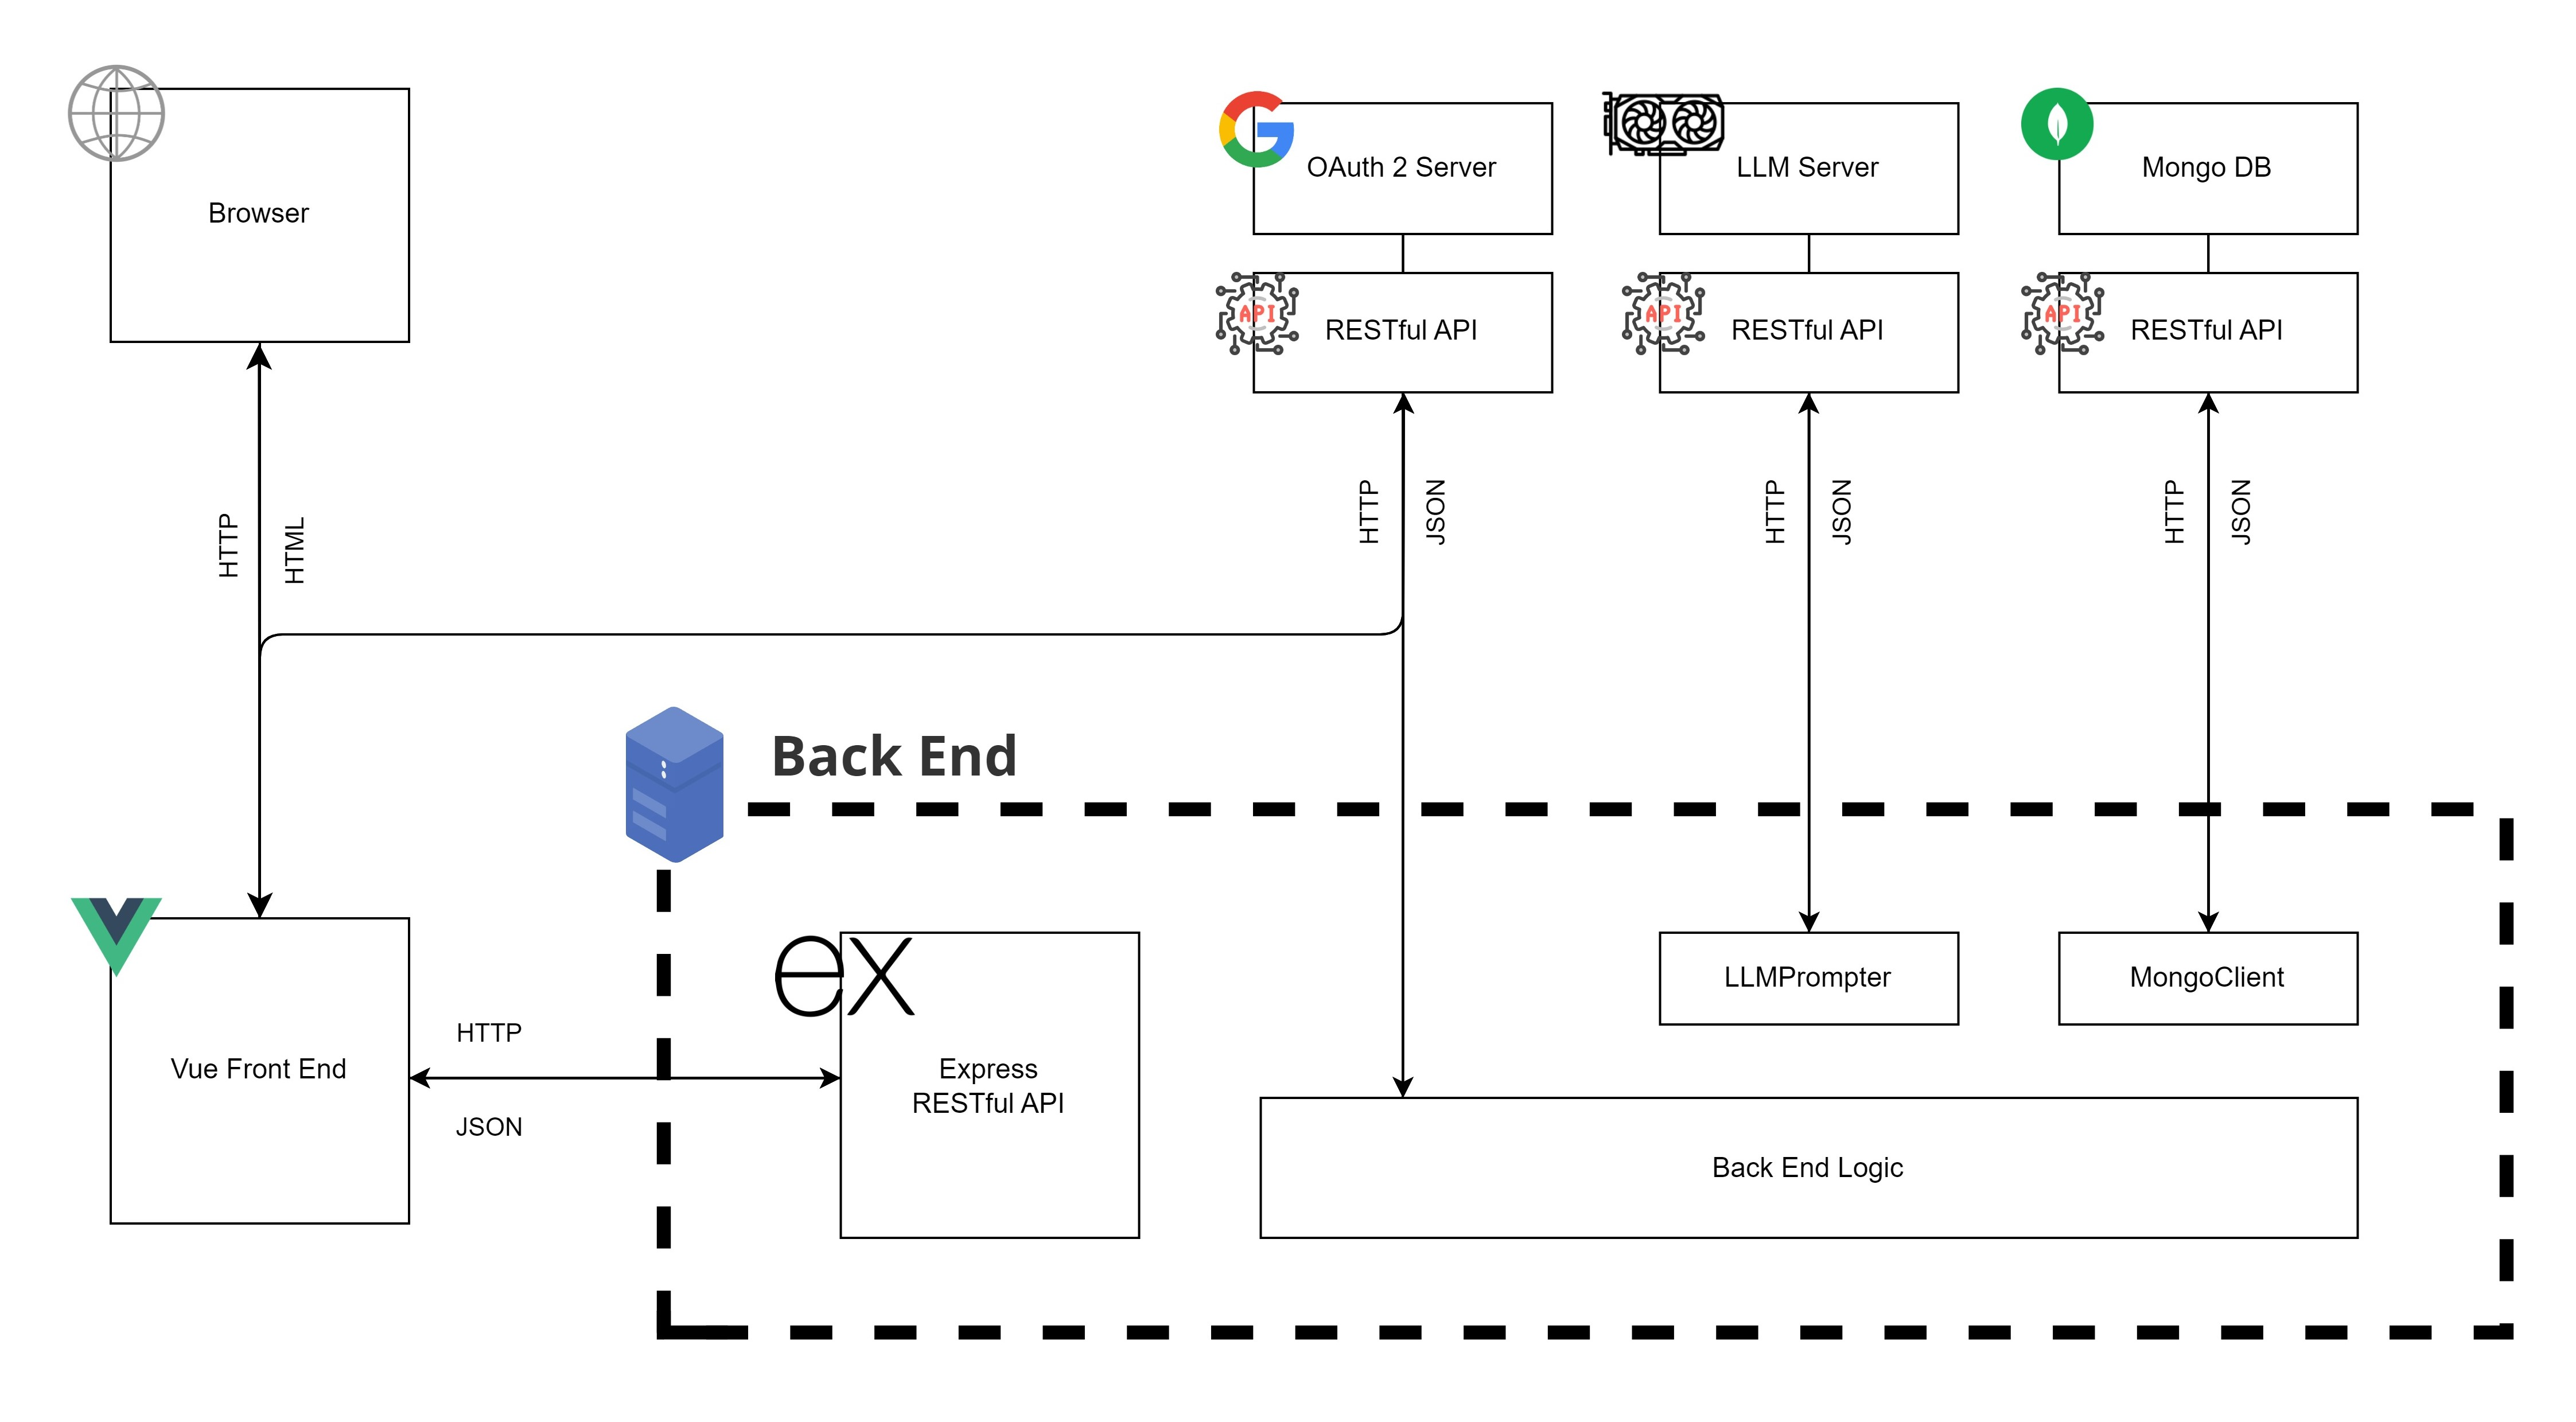
\includegraphics[width=0.95\textwidth]{images/architecture.jpg}
  \caption{\small The architecture diagram ot the MindMerge system}
\end{figure}
The architecture is relatively simple,
comprising two classical components: the front end and the back end, along with several smaller components (browser, OAuth server, LLM service, and MongoDB).
\newline \newline
The browser communicates with the front end using the HTTP protocol and HTML format.
\newline \newline
The front end, based on the Vue library, accesses resources provided by the back end using HTTP with JSON data format.
\newline \newline
Authentication is provided by a third-party OAuth server, that communicate with both the front end and back end via HTTP/JSON.
\newline \newline
The back end is the most complex component consists of several sub-components, including:
\begin{itemize}
  \item A part providing RESTful APIs based on Express.js
  \item A component dedicated to communicating with the database (MongoClient)
  \item A module for communicating with the LLM service (LLMPrompter)
  \item Logic containing all functions necessary for the application's operation.
\end{itemize}
All the communications that the backend has with the external world are made through HTTP with json format.

\section{Product Backlog}


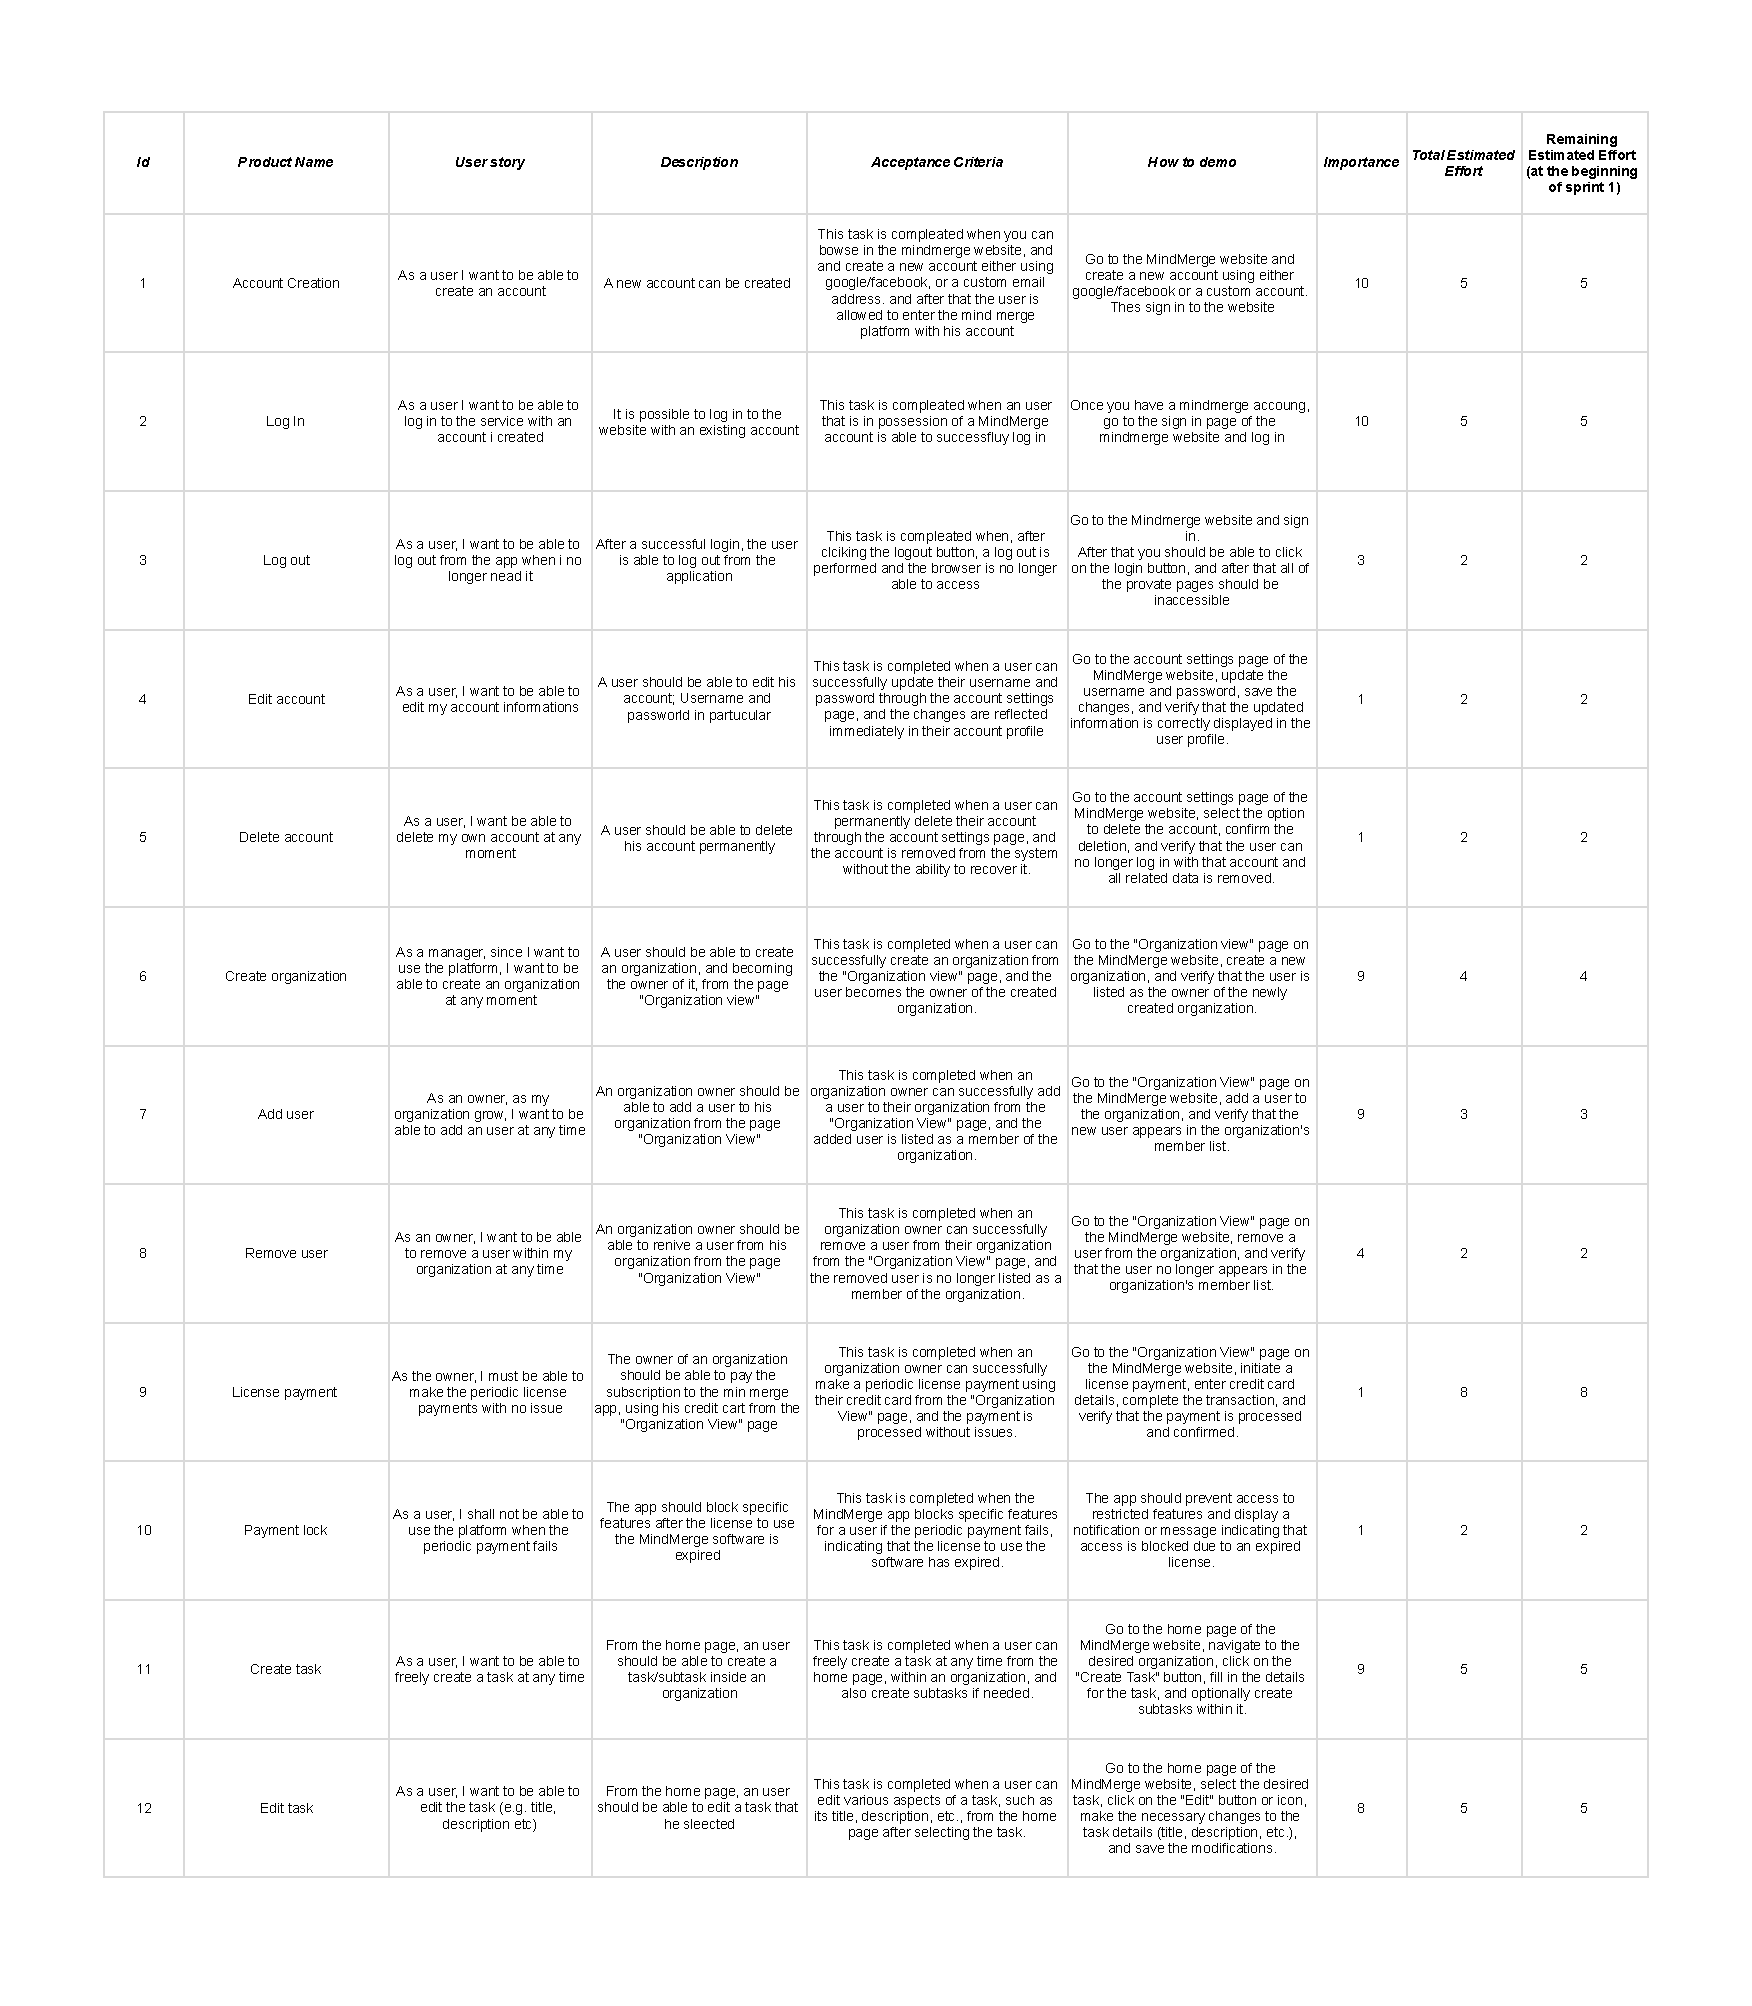
\includepdf[pages=-]{images/product_backlog.pdf}

\section{Definition of Tests}

\subsection*{Test DatabaseManager:TaskManager}
This section contains the tests for the TaskManager class, which is responsible for managing tasks in the database.
\newline
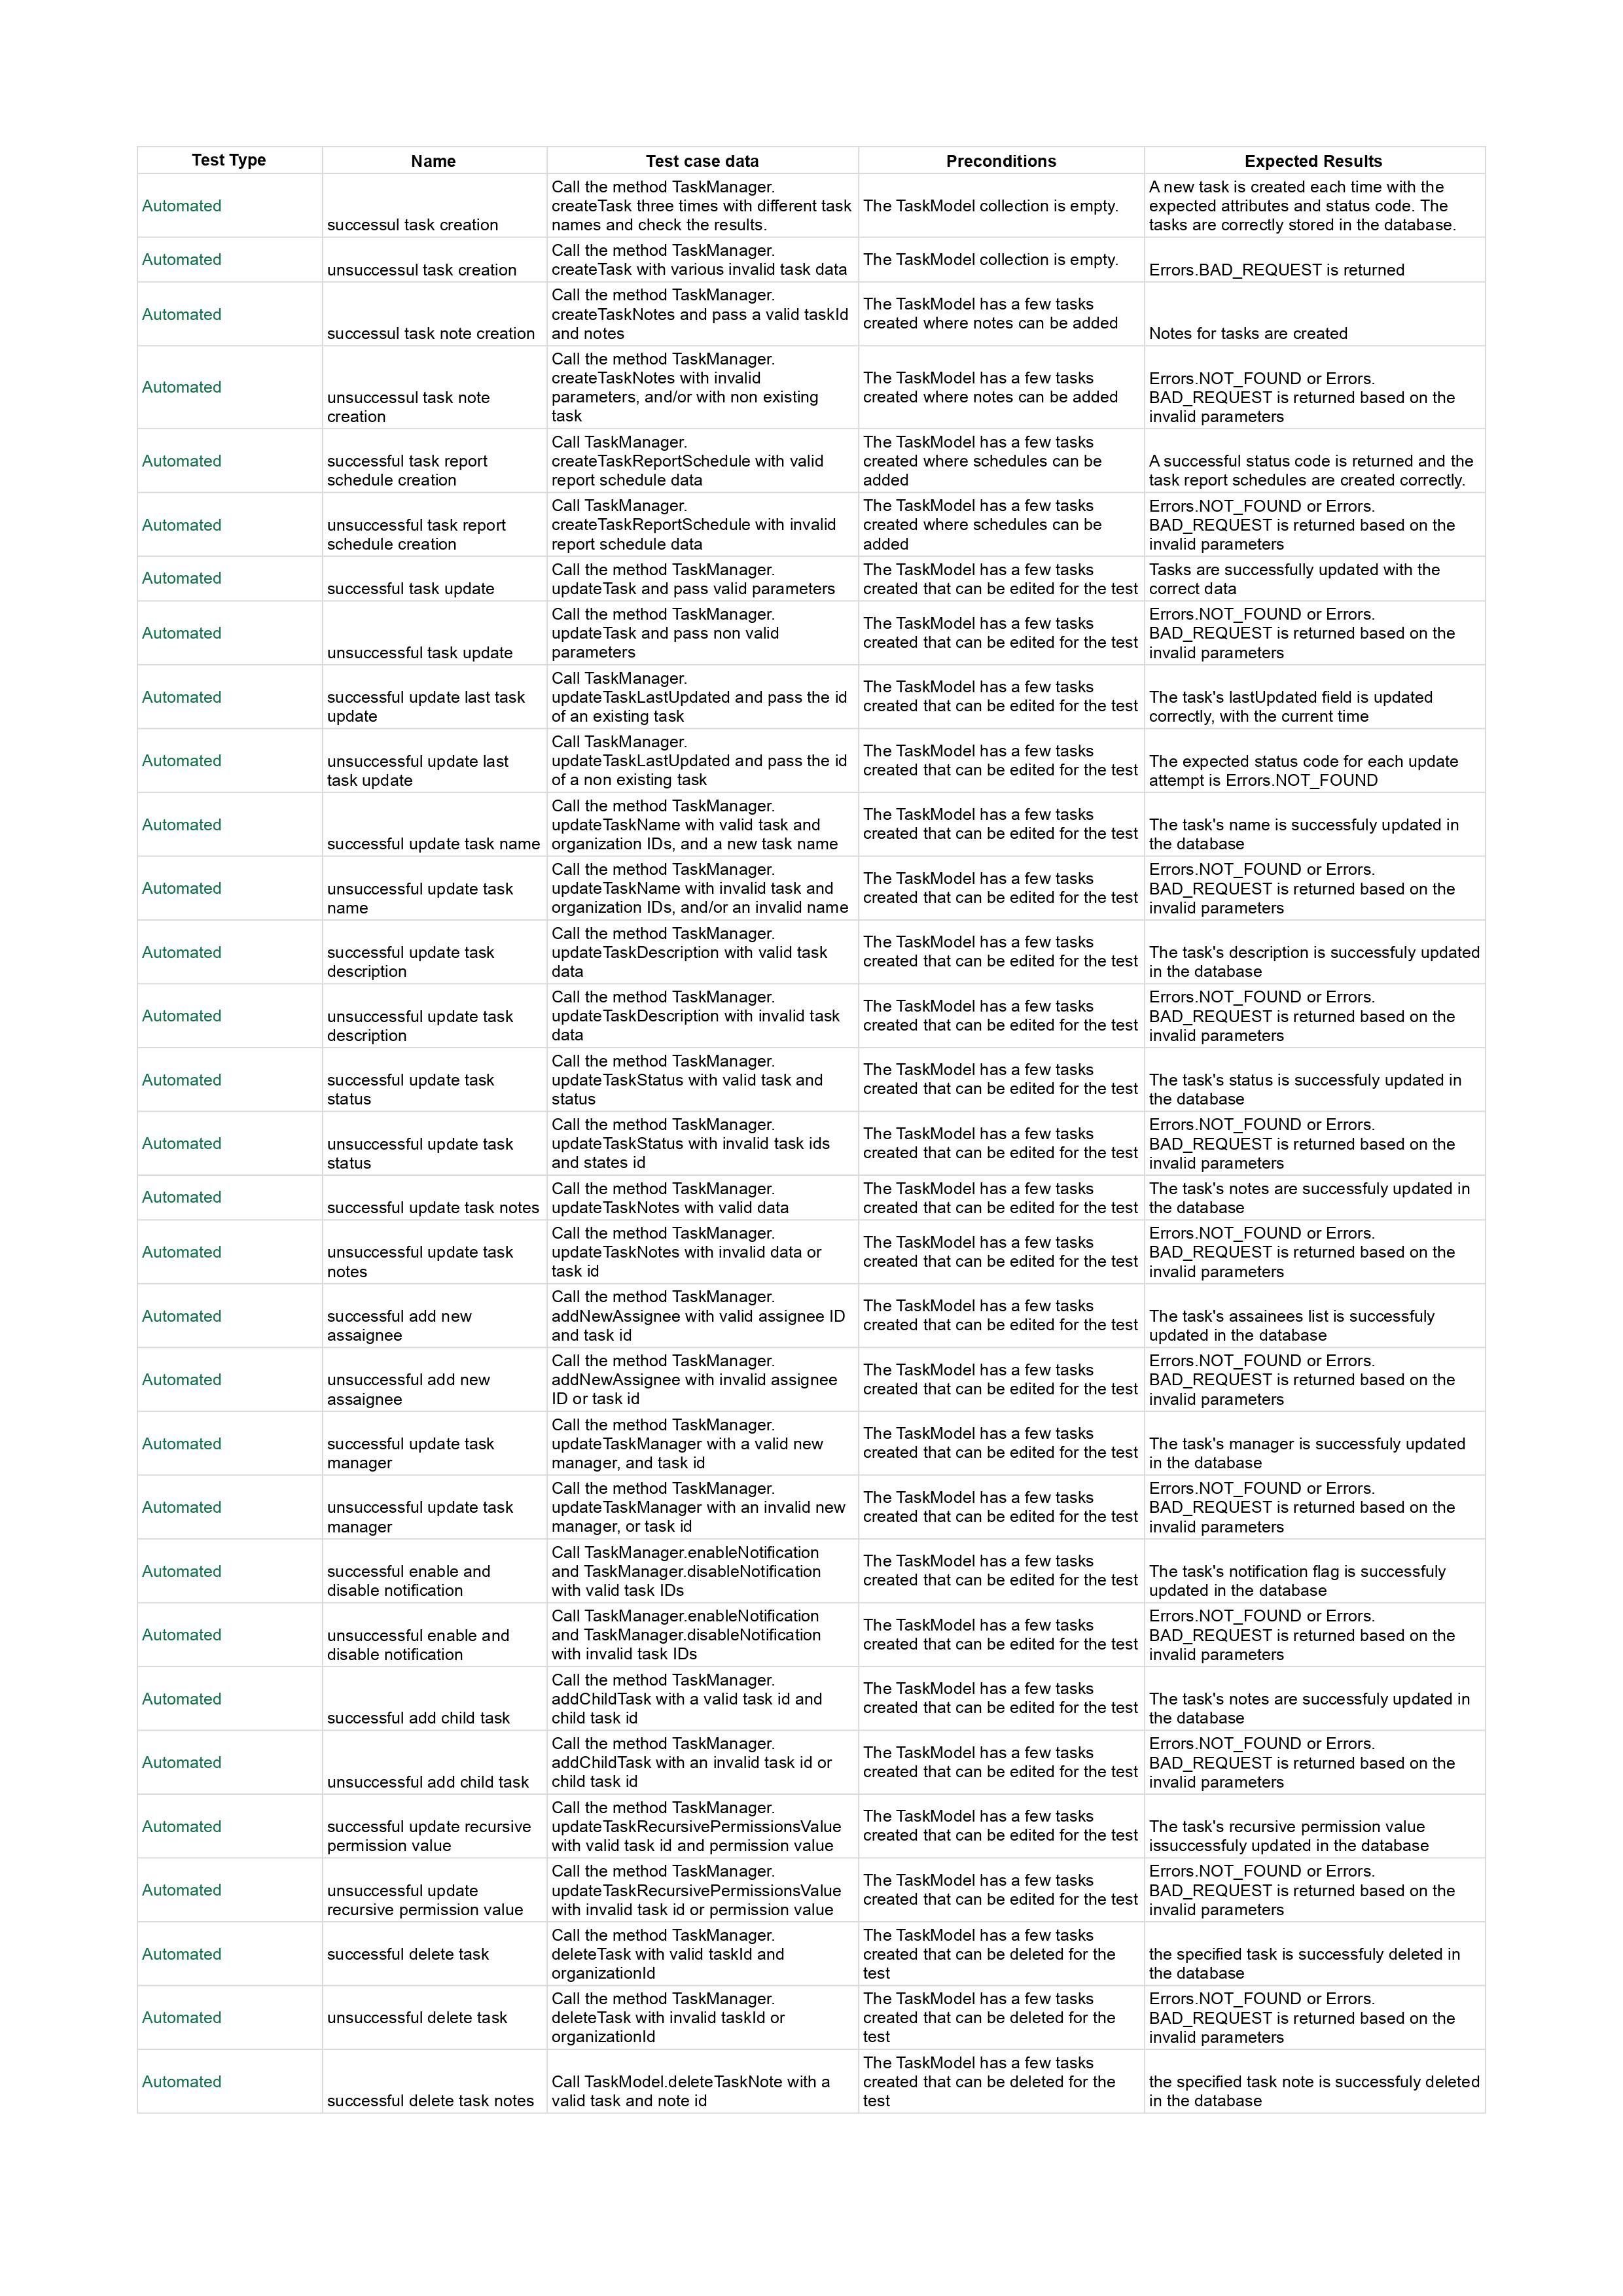
\includegraphics[width=0.95\textwidth]{images/Test_DatabaseManagerTaskManager-immagini-0.jpg}
\newline
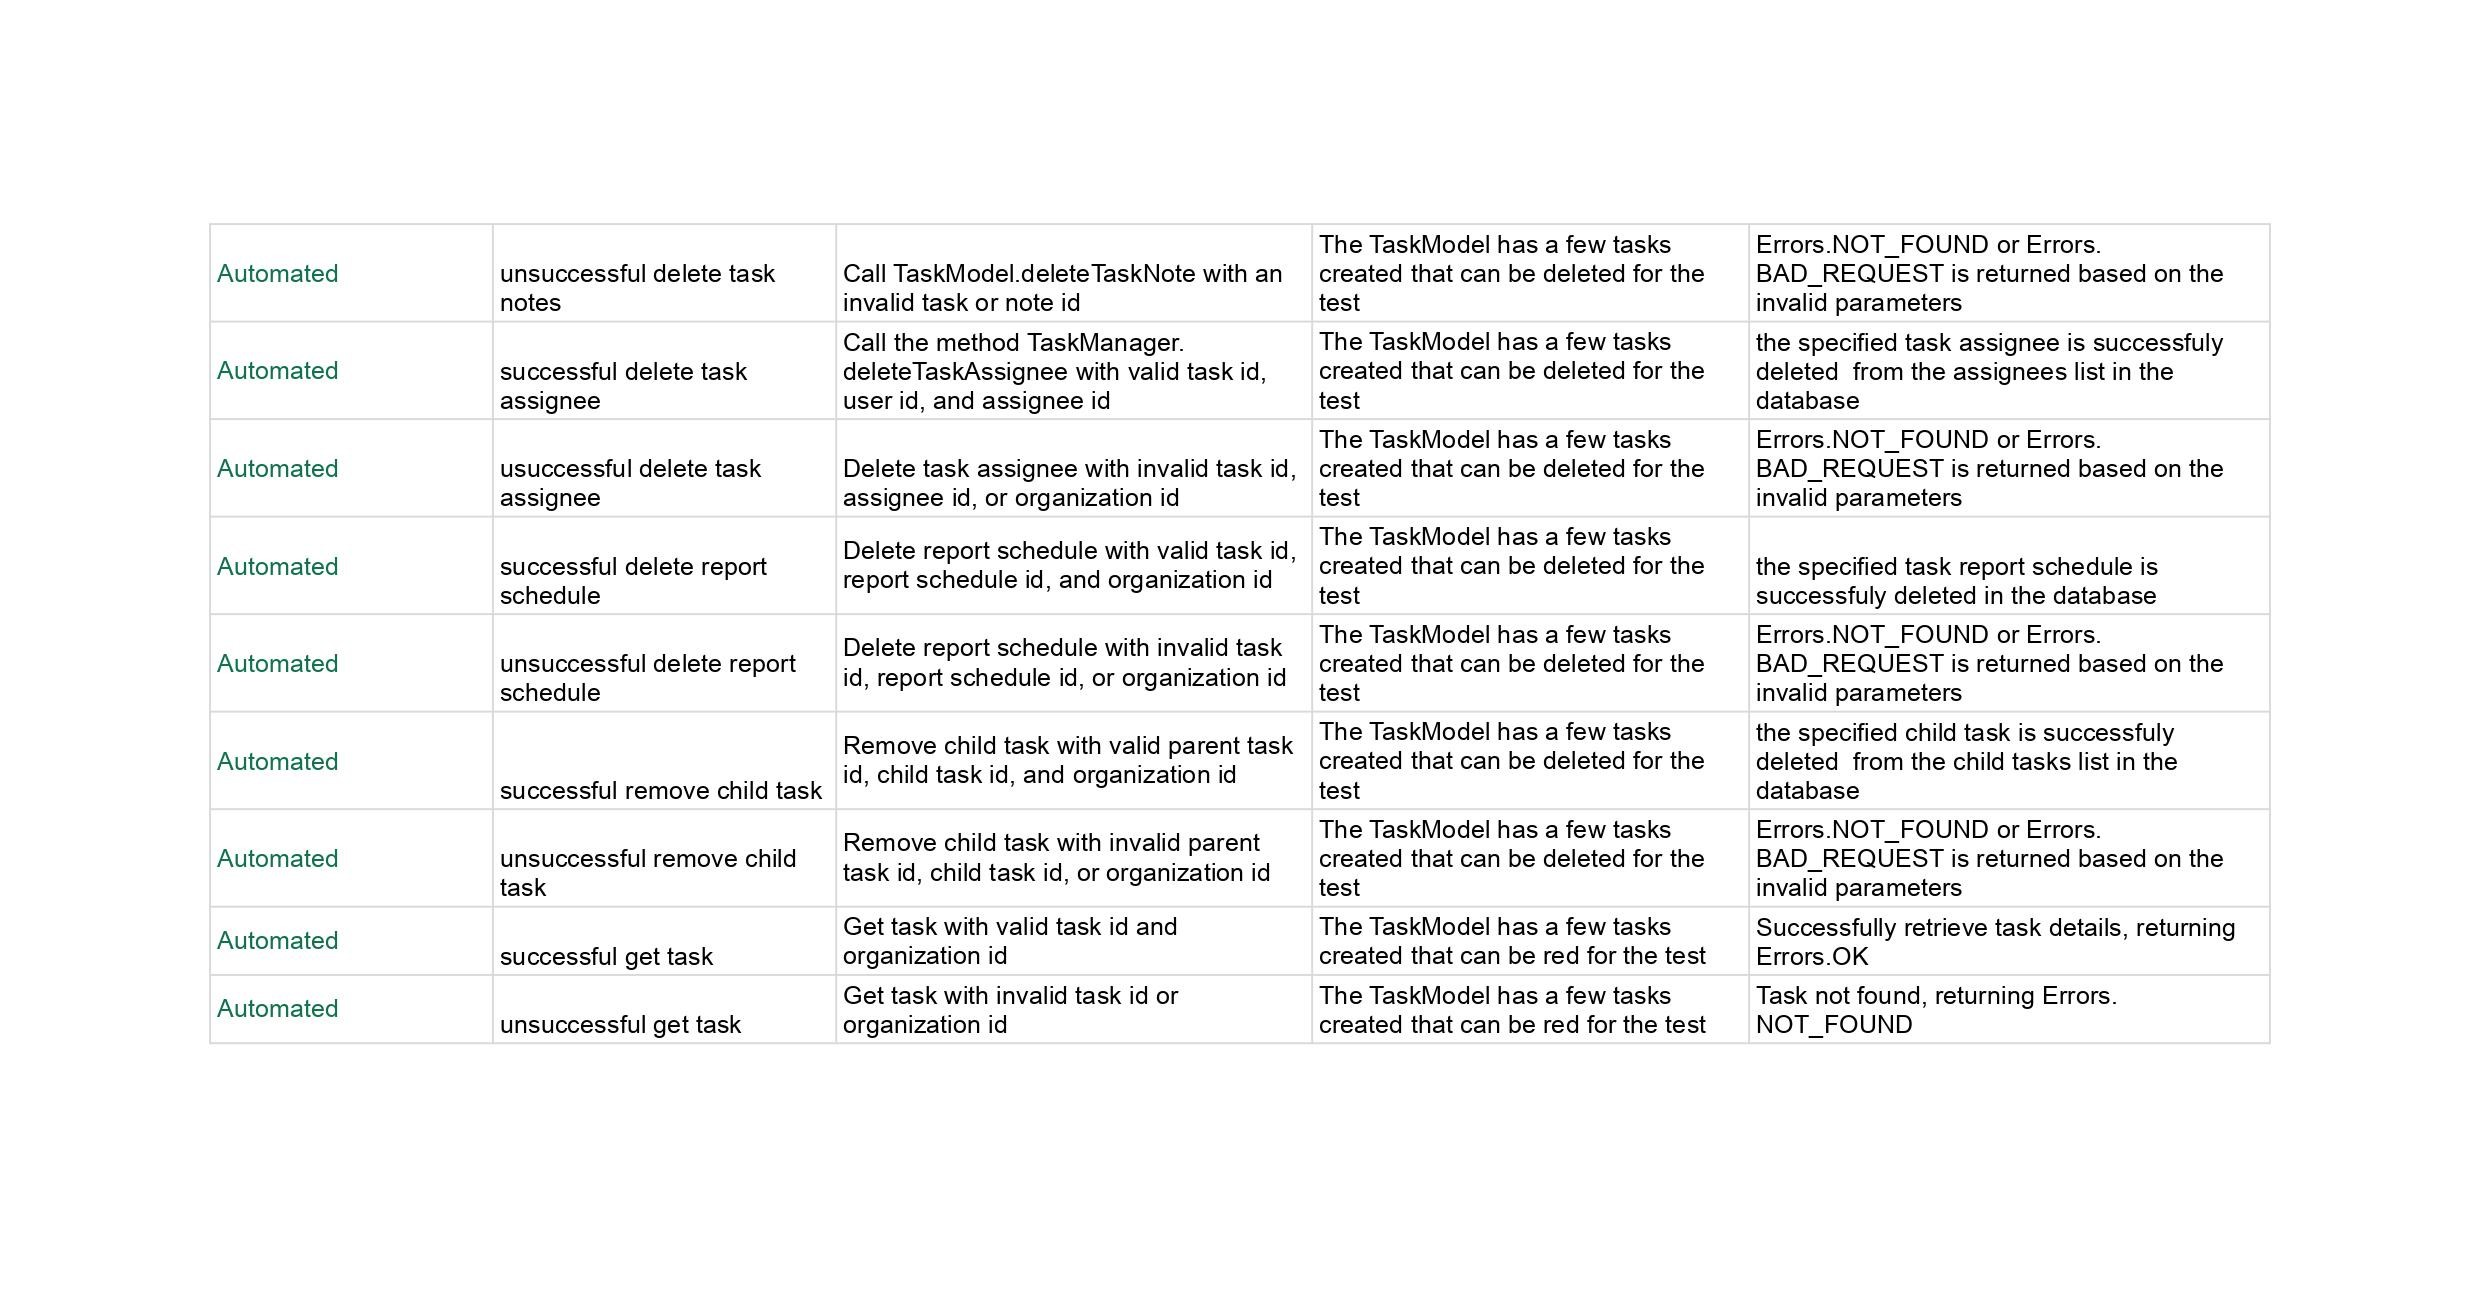
\includegraphics[width=0.95\textwidth]{images/Test_DatabaseManagerTaskManager-immagini-1.jpg}
\subsection*{Test OrganizationManager}
This section is dedicated to the tests for the OrganizationManager class, which is responsible for managing organizations in the database, with the integrated API.
\newline
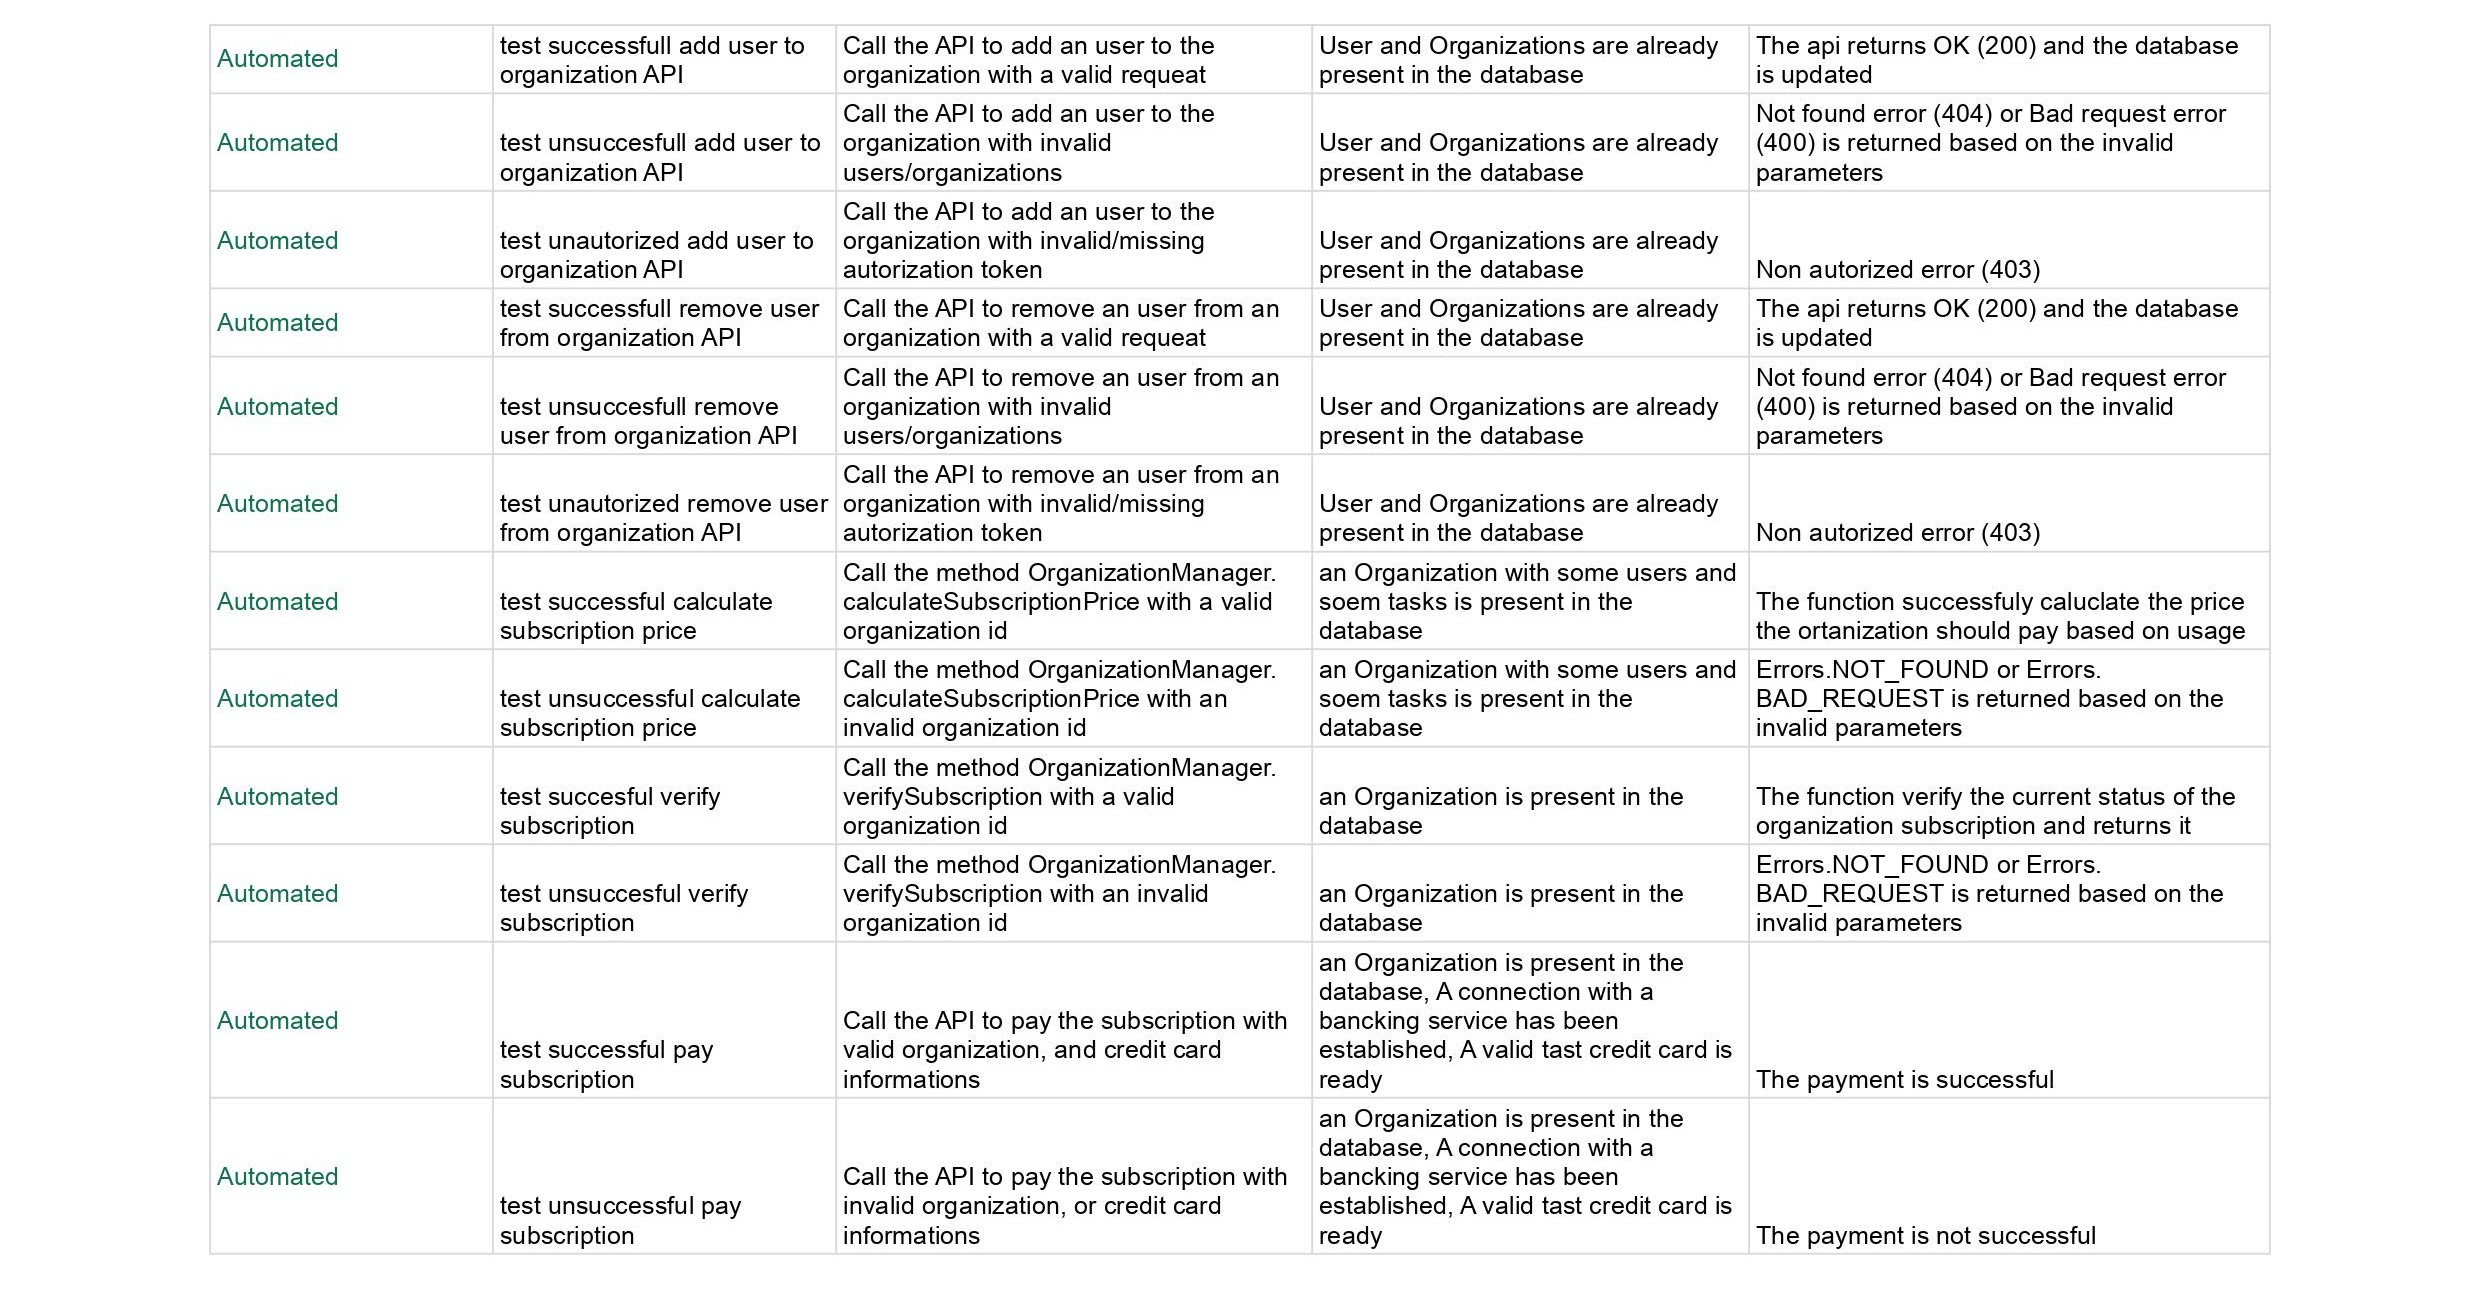
\includegraphics[width=0.95\textwidth]{images/Test_OrganizationManager.jpg}

\subsection*{Test Report Page}
This section includes manual tests for the Report Page, which is responsible for generating reports.
\newline
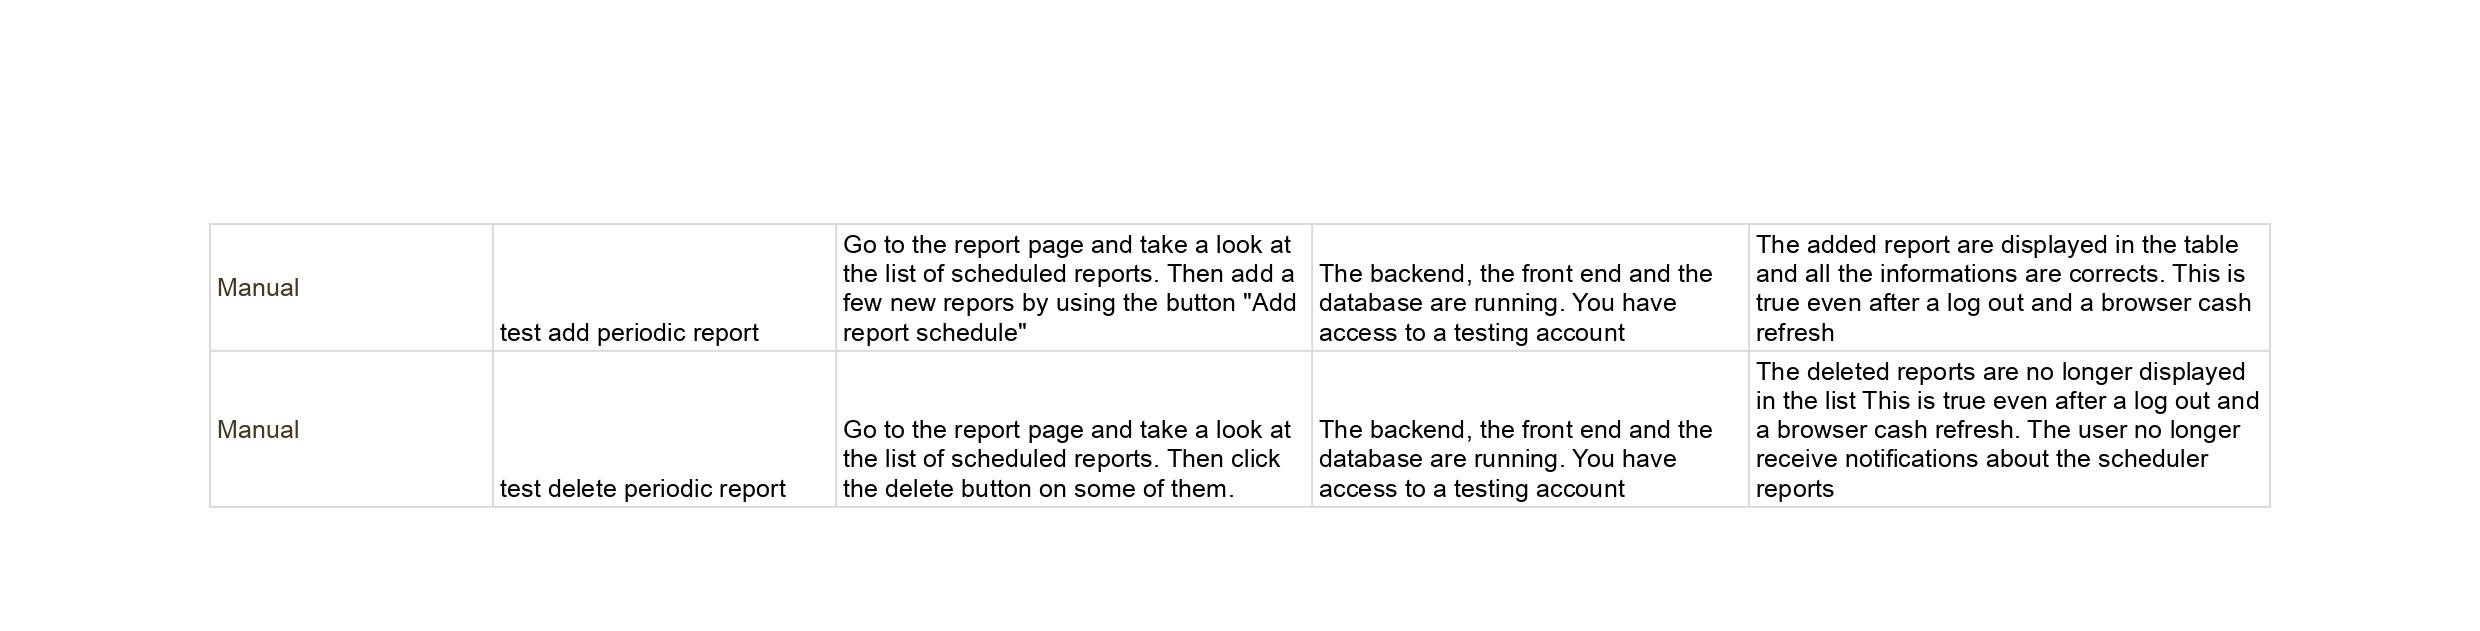
\includegraphics[width=0.95\textwidth]{images/Test_ReportPage.jpg}
\subsection*{Test NotificationManager}
This section includes automated tests for the NotificationManager class, which is responsible for managing notifications in the database.
\newline
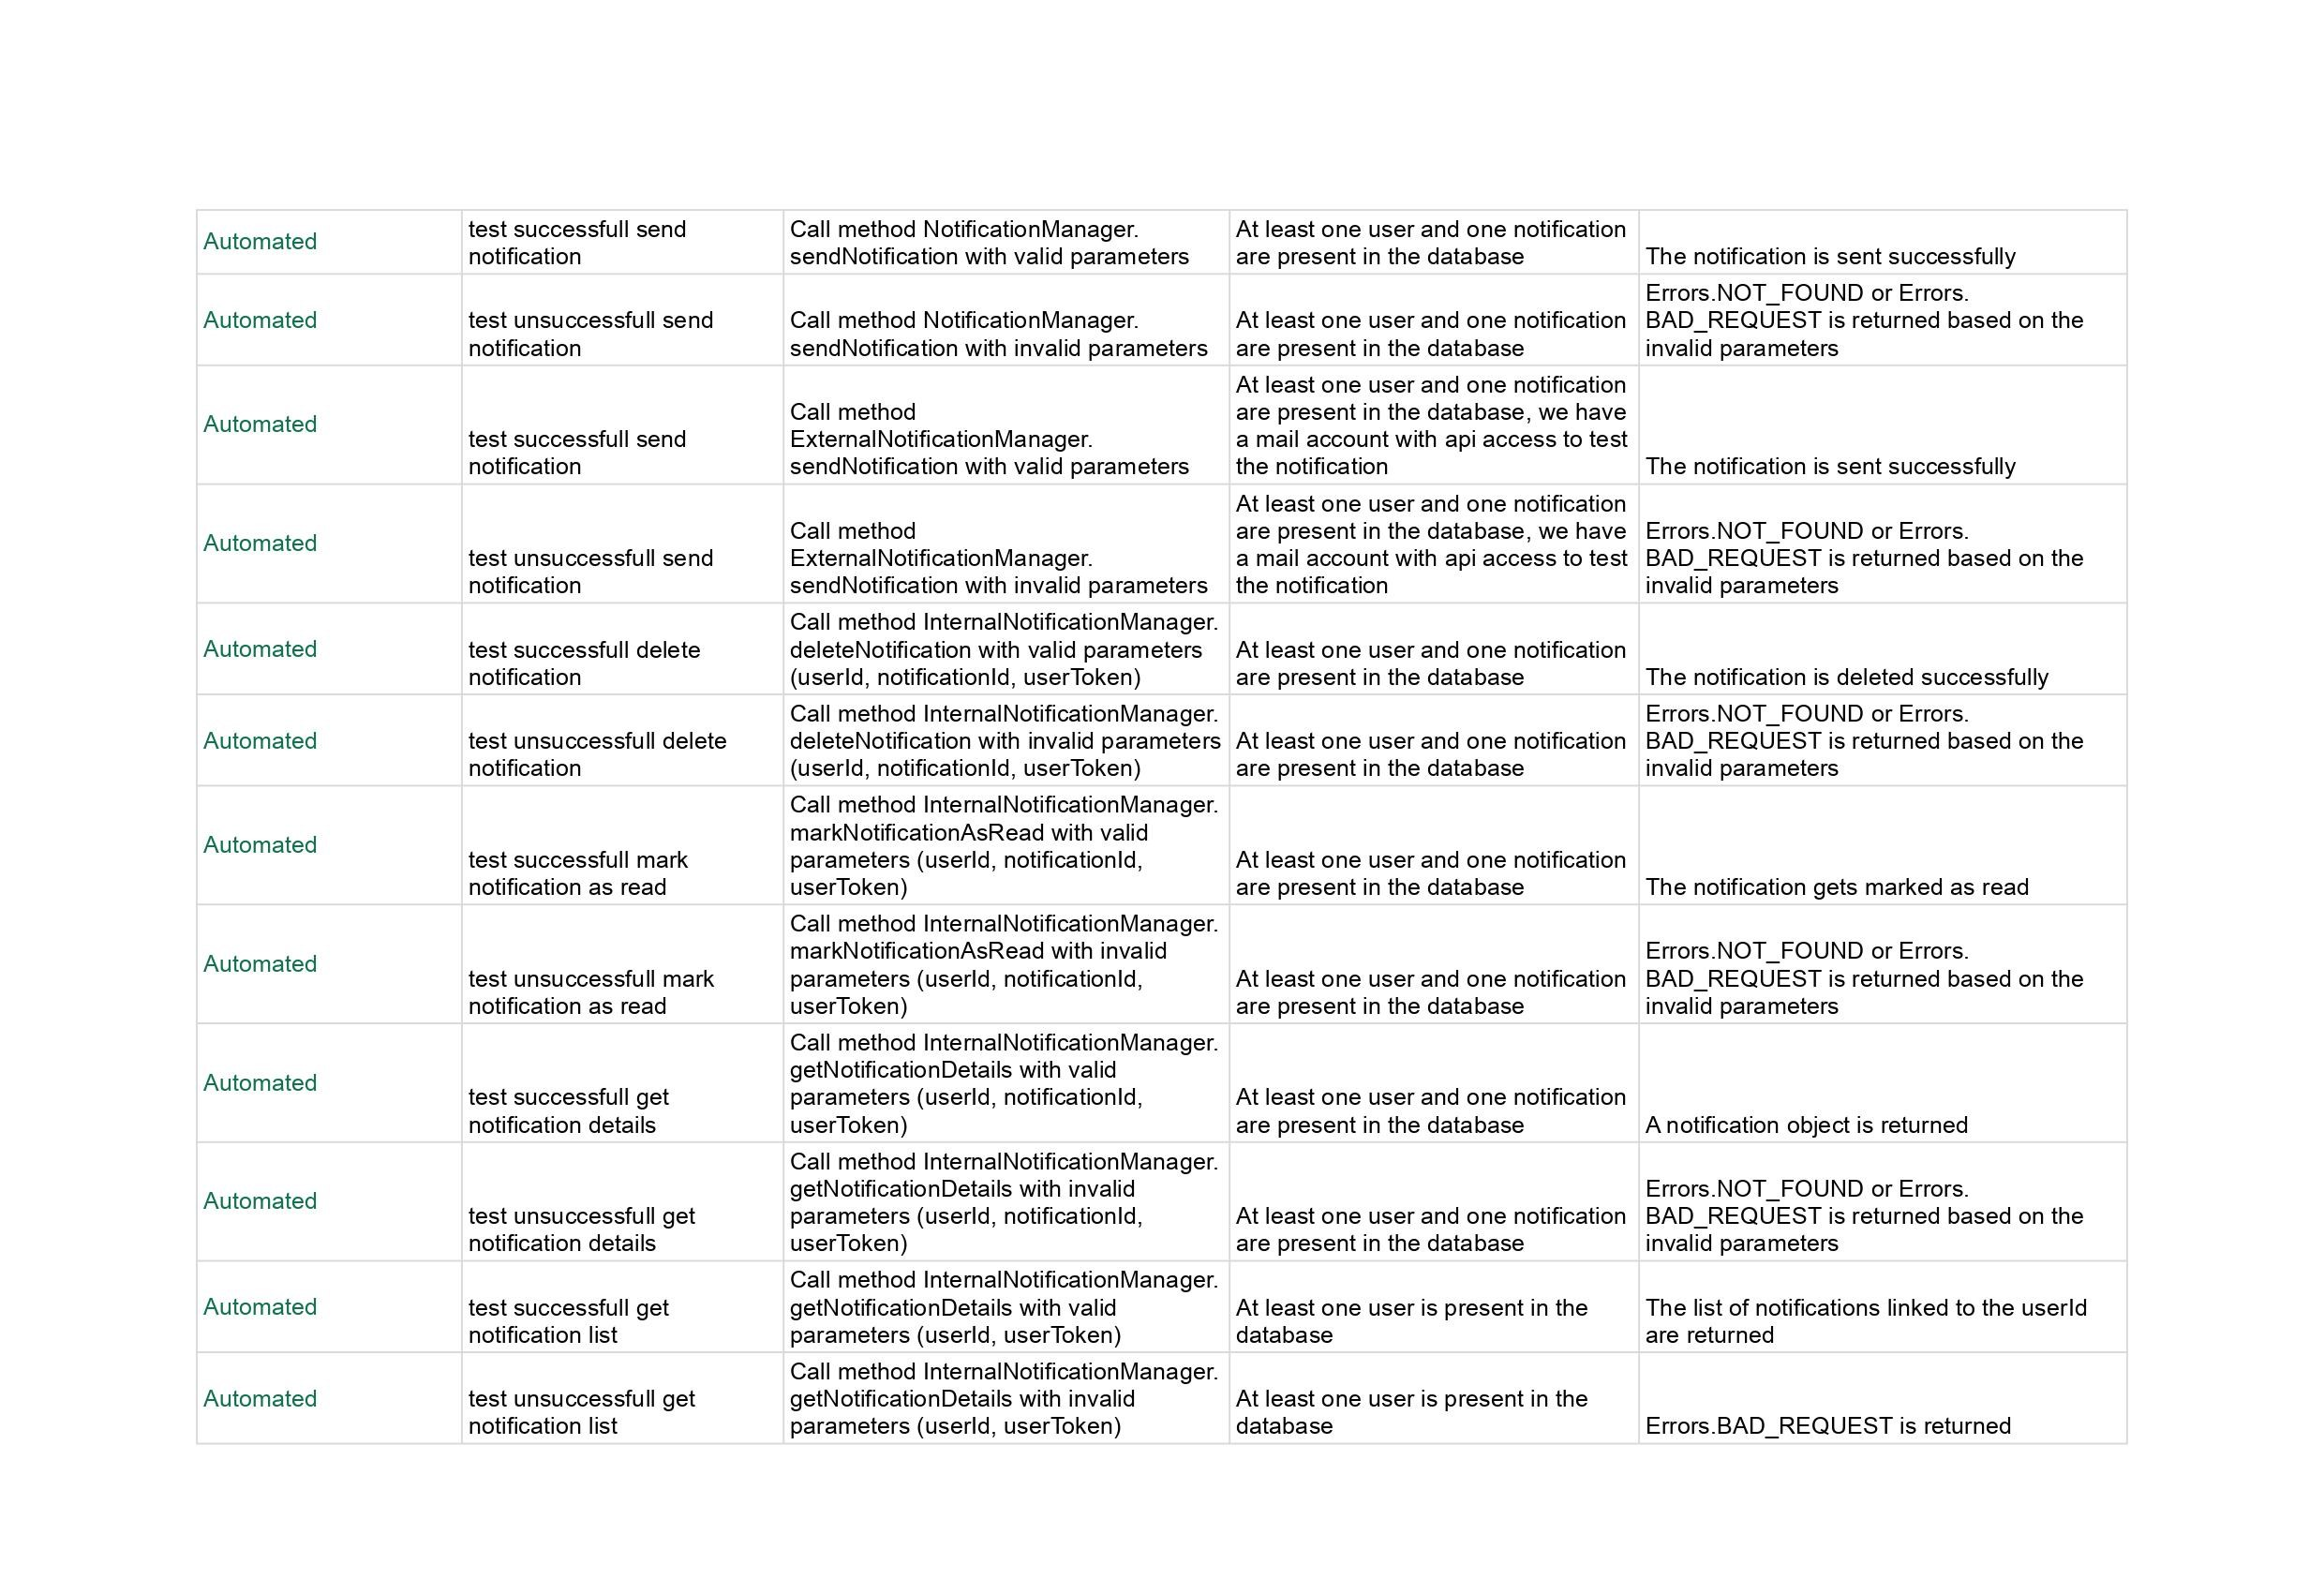
\includegraphics[width=0.95\textwidth]{images/Test_NotificationManager.jpg}

\subsection*{Test ReportManager}
This section includes automated tests for the ReportManager class, which is responsible for managing reports in the database.
\newline
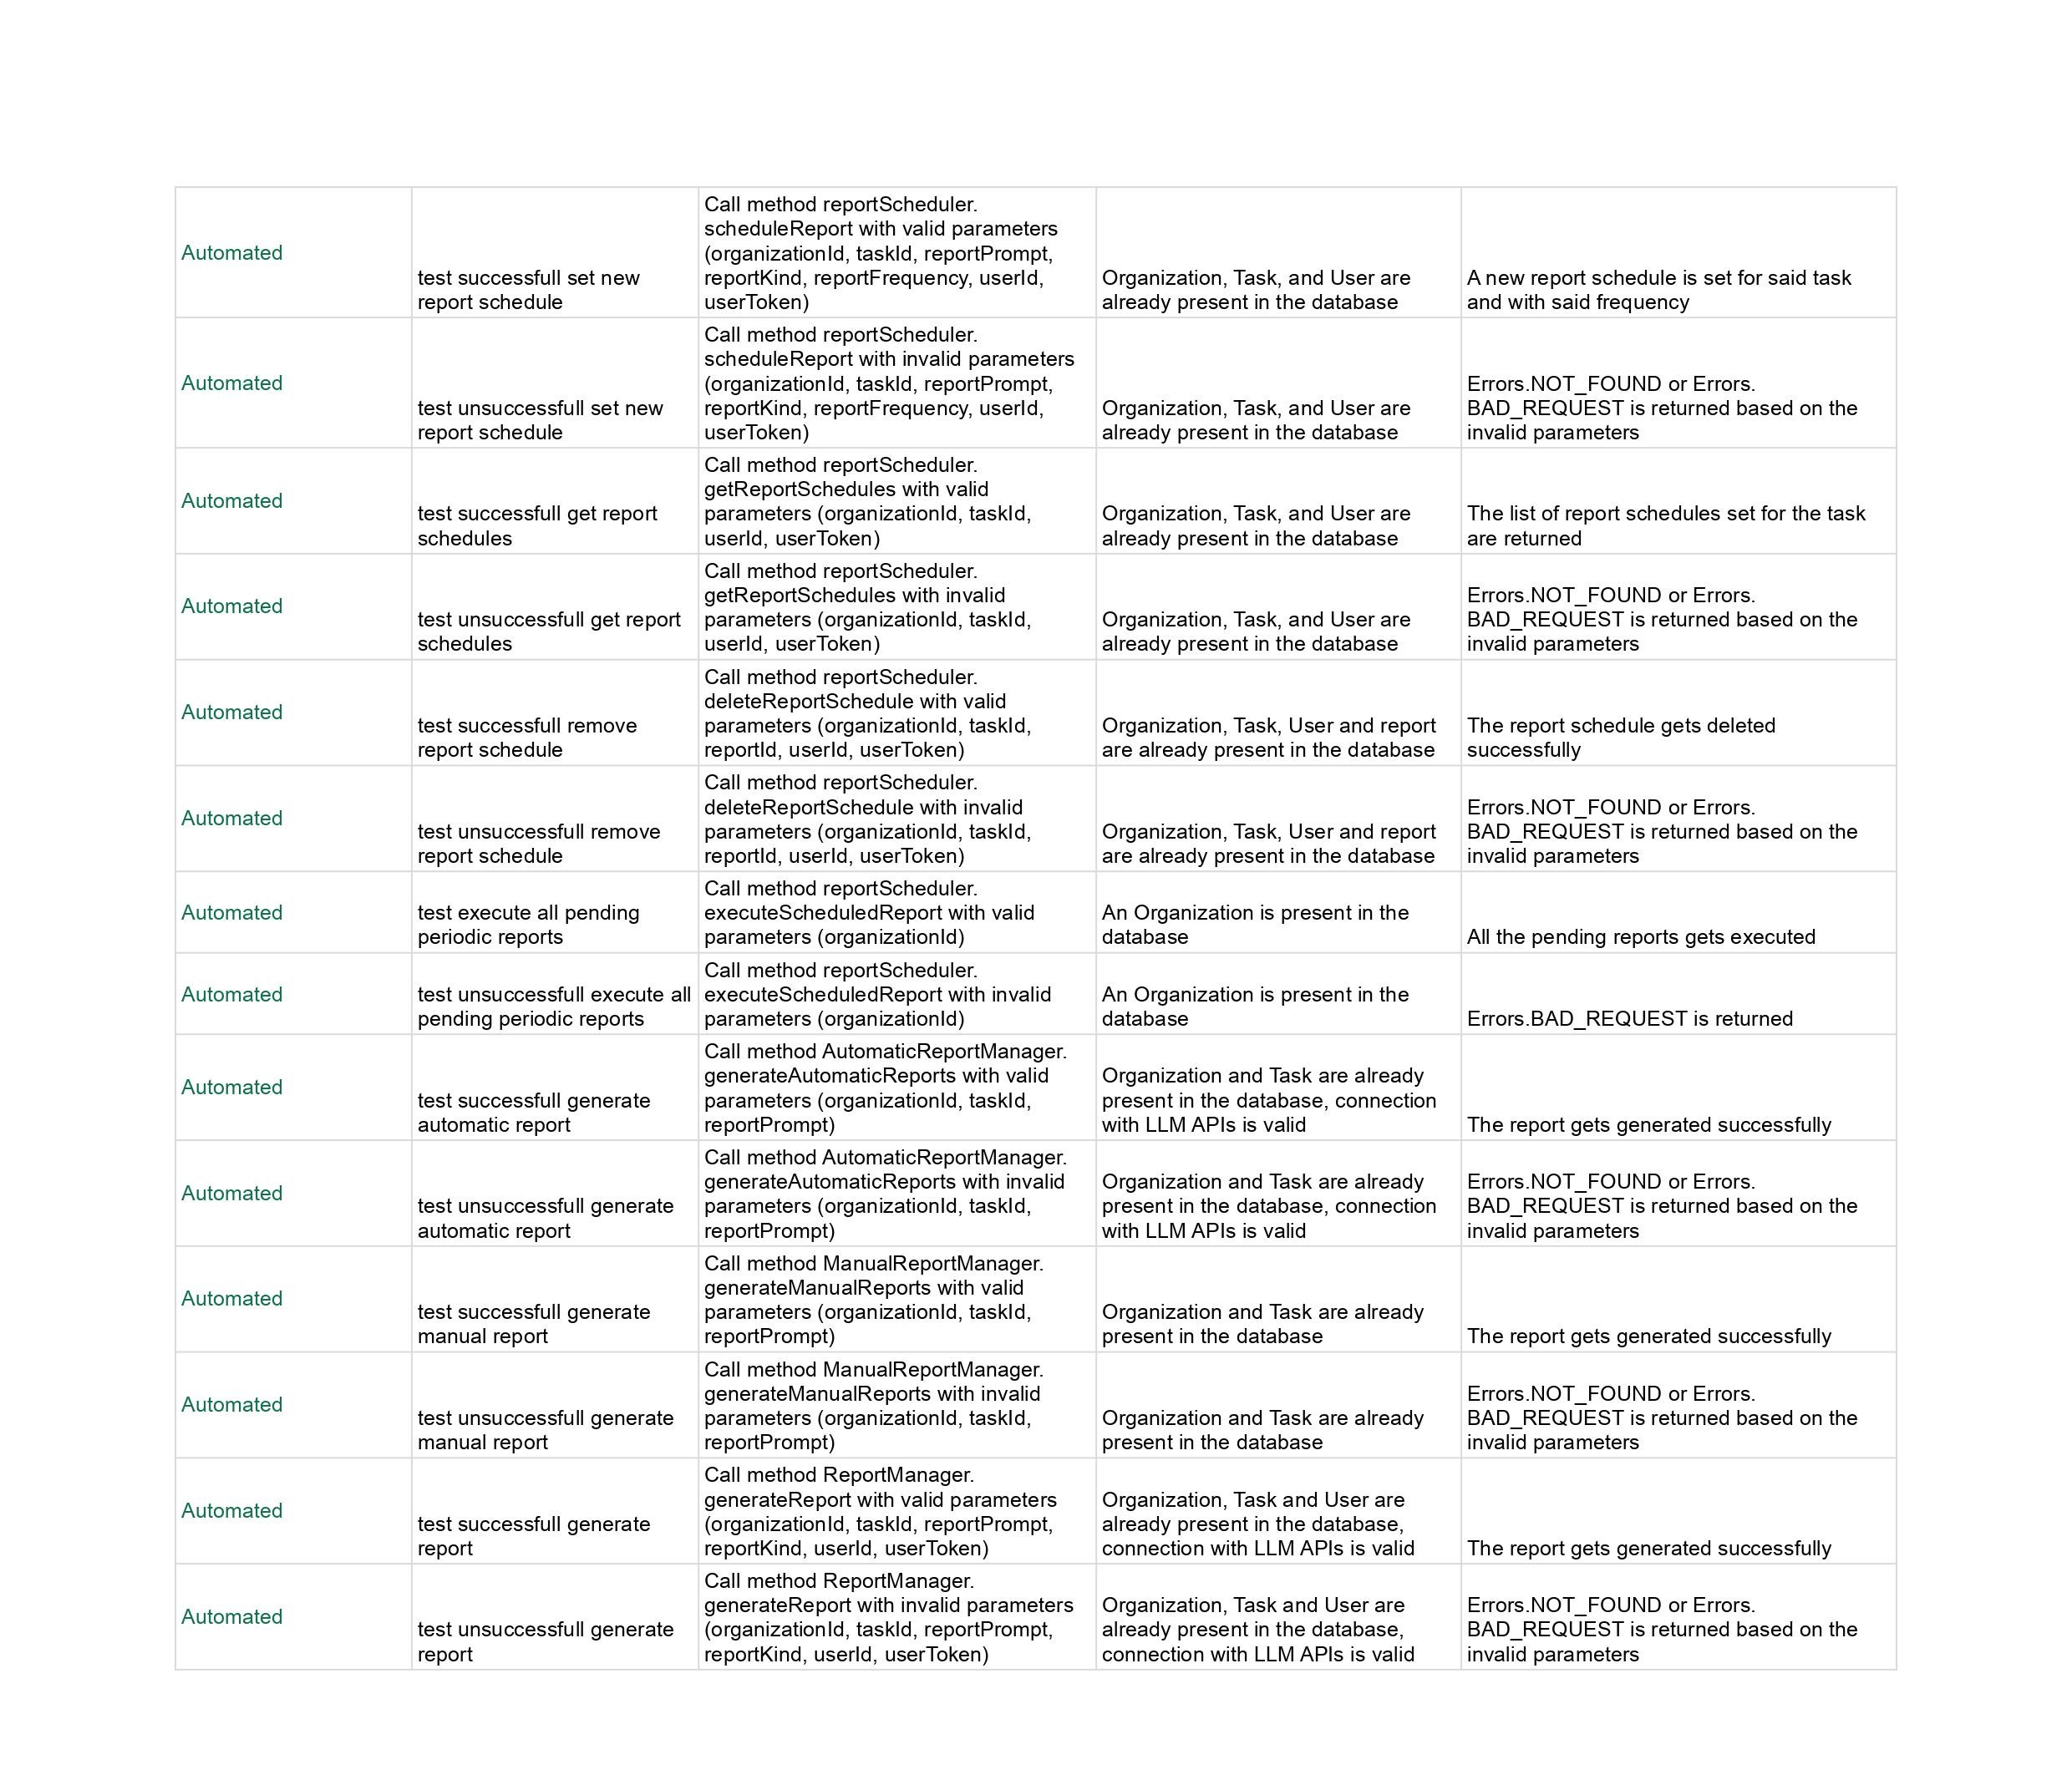
\includegraphics[width=0.95\textwidth]{images/Test_ReportManager.jpg}

\subsection*{Test DatabaseManager::OrganizationManager}
This section is dedicated to the tests for the OrganizationManager class, which is responsible for managing organizations in the database.
\newline
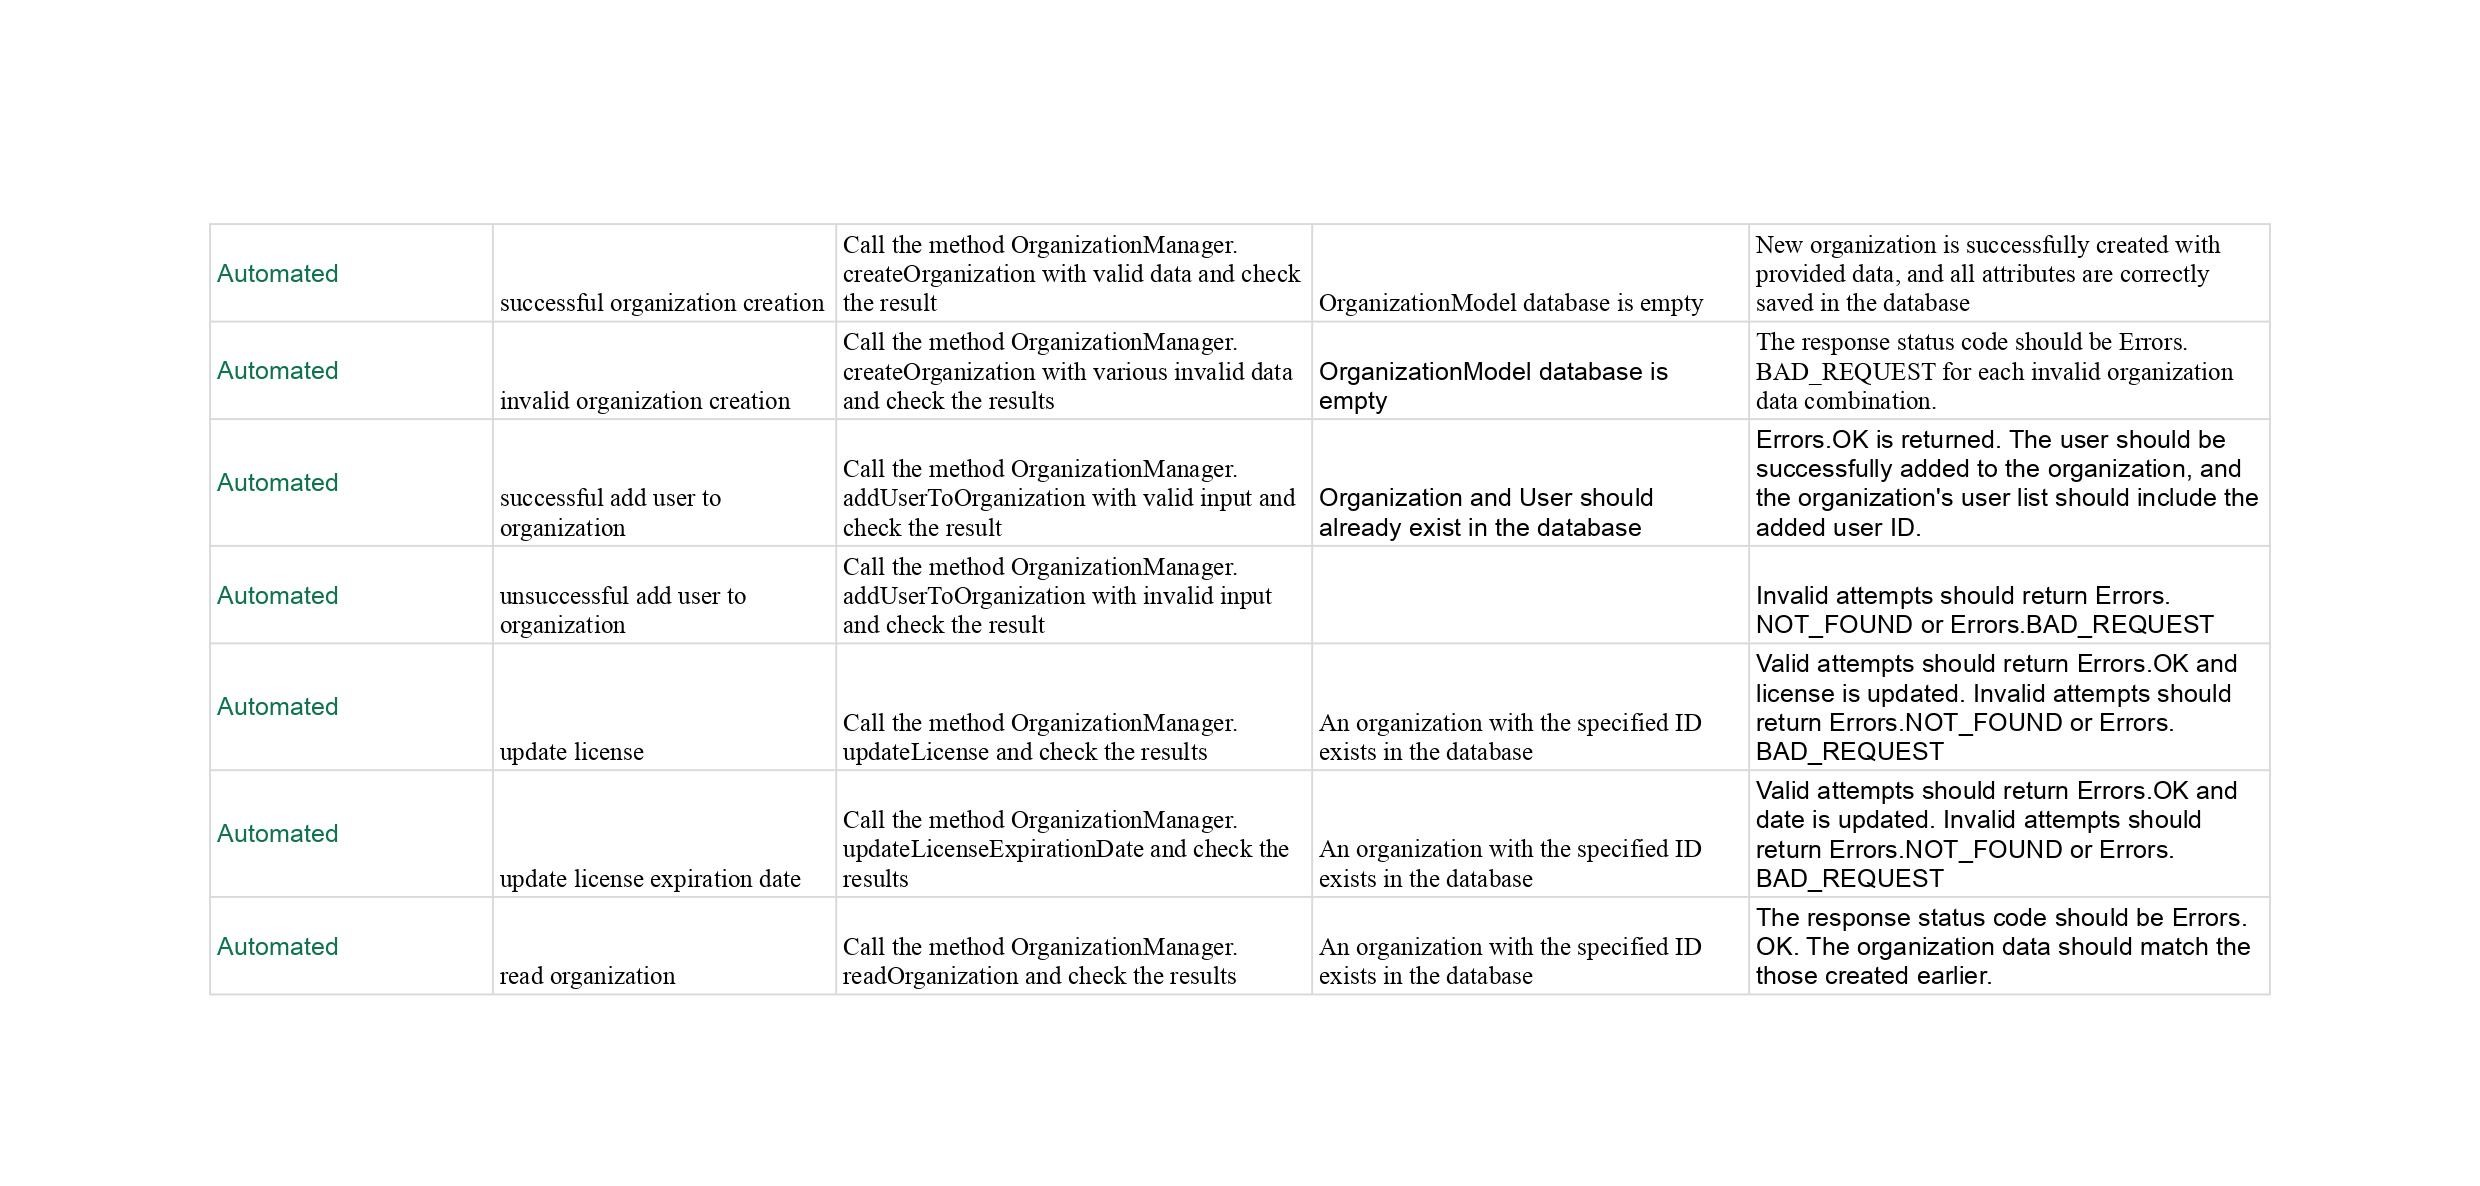
\includegraphics[width=0.95\textwidth]{images/Test_DatabaseManagerOrganizationManager.jpg}

\subsection*{Test AccountManager}
This section includes automated tests for the AccountManager class, which is responsible for managing accounts in the database.
\newline
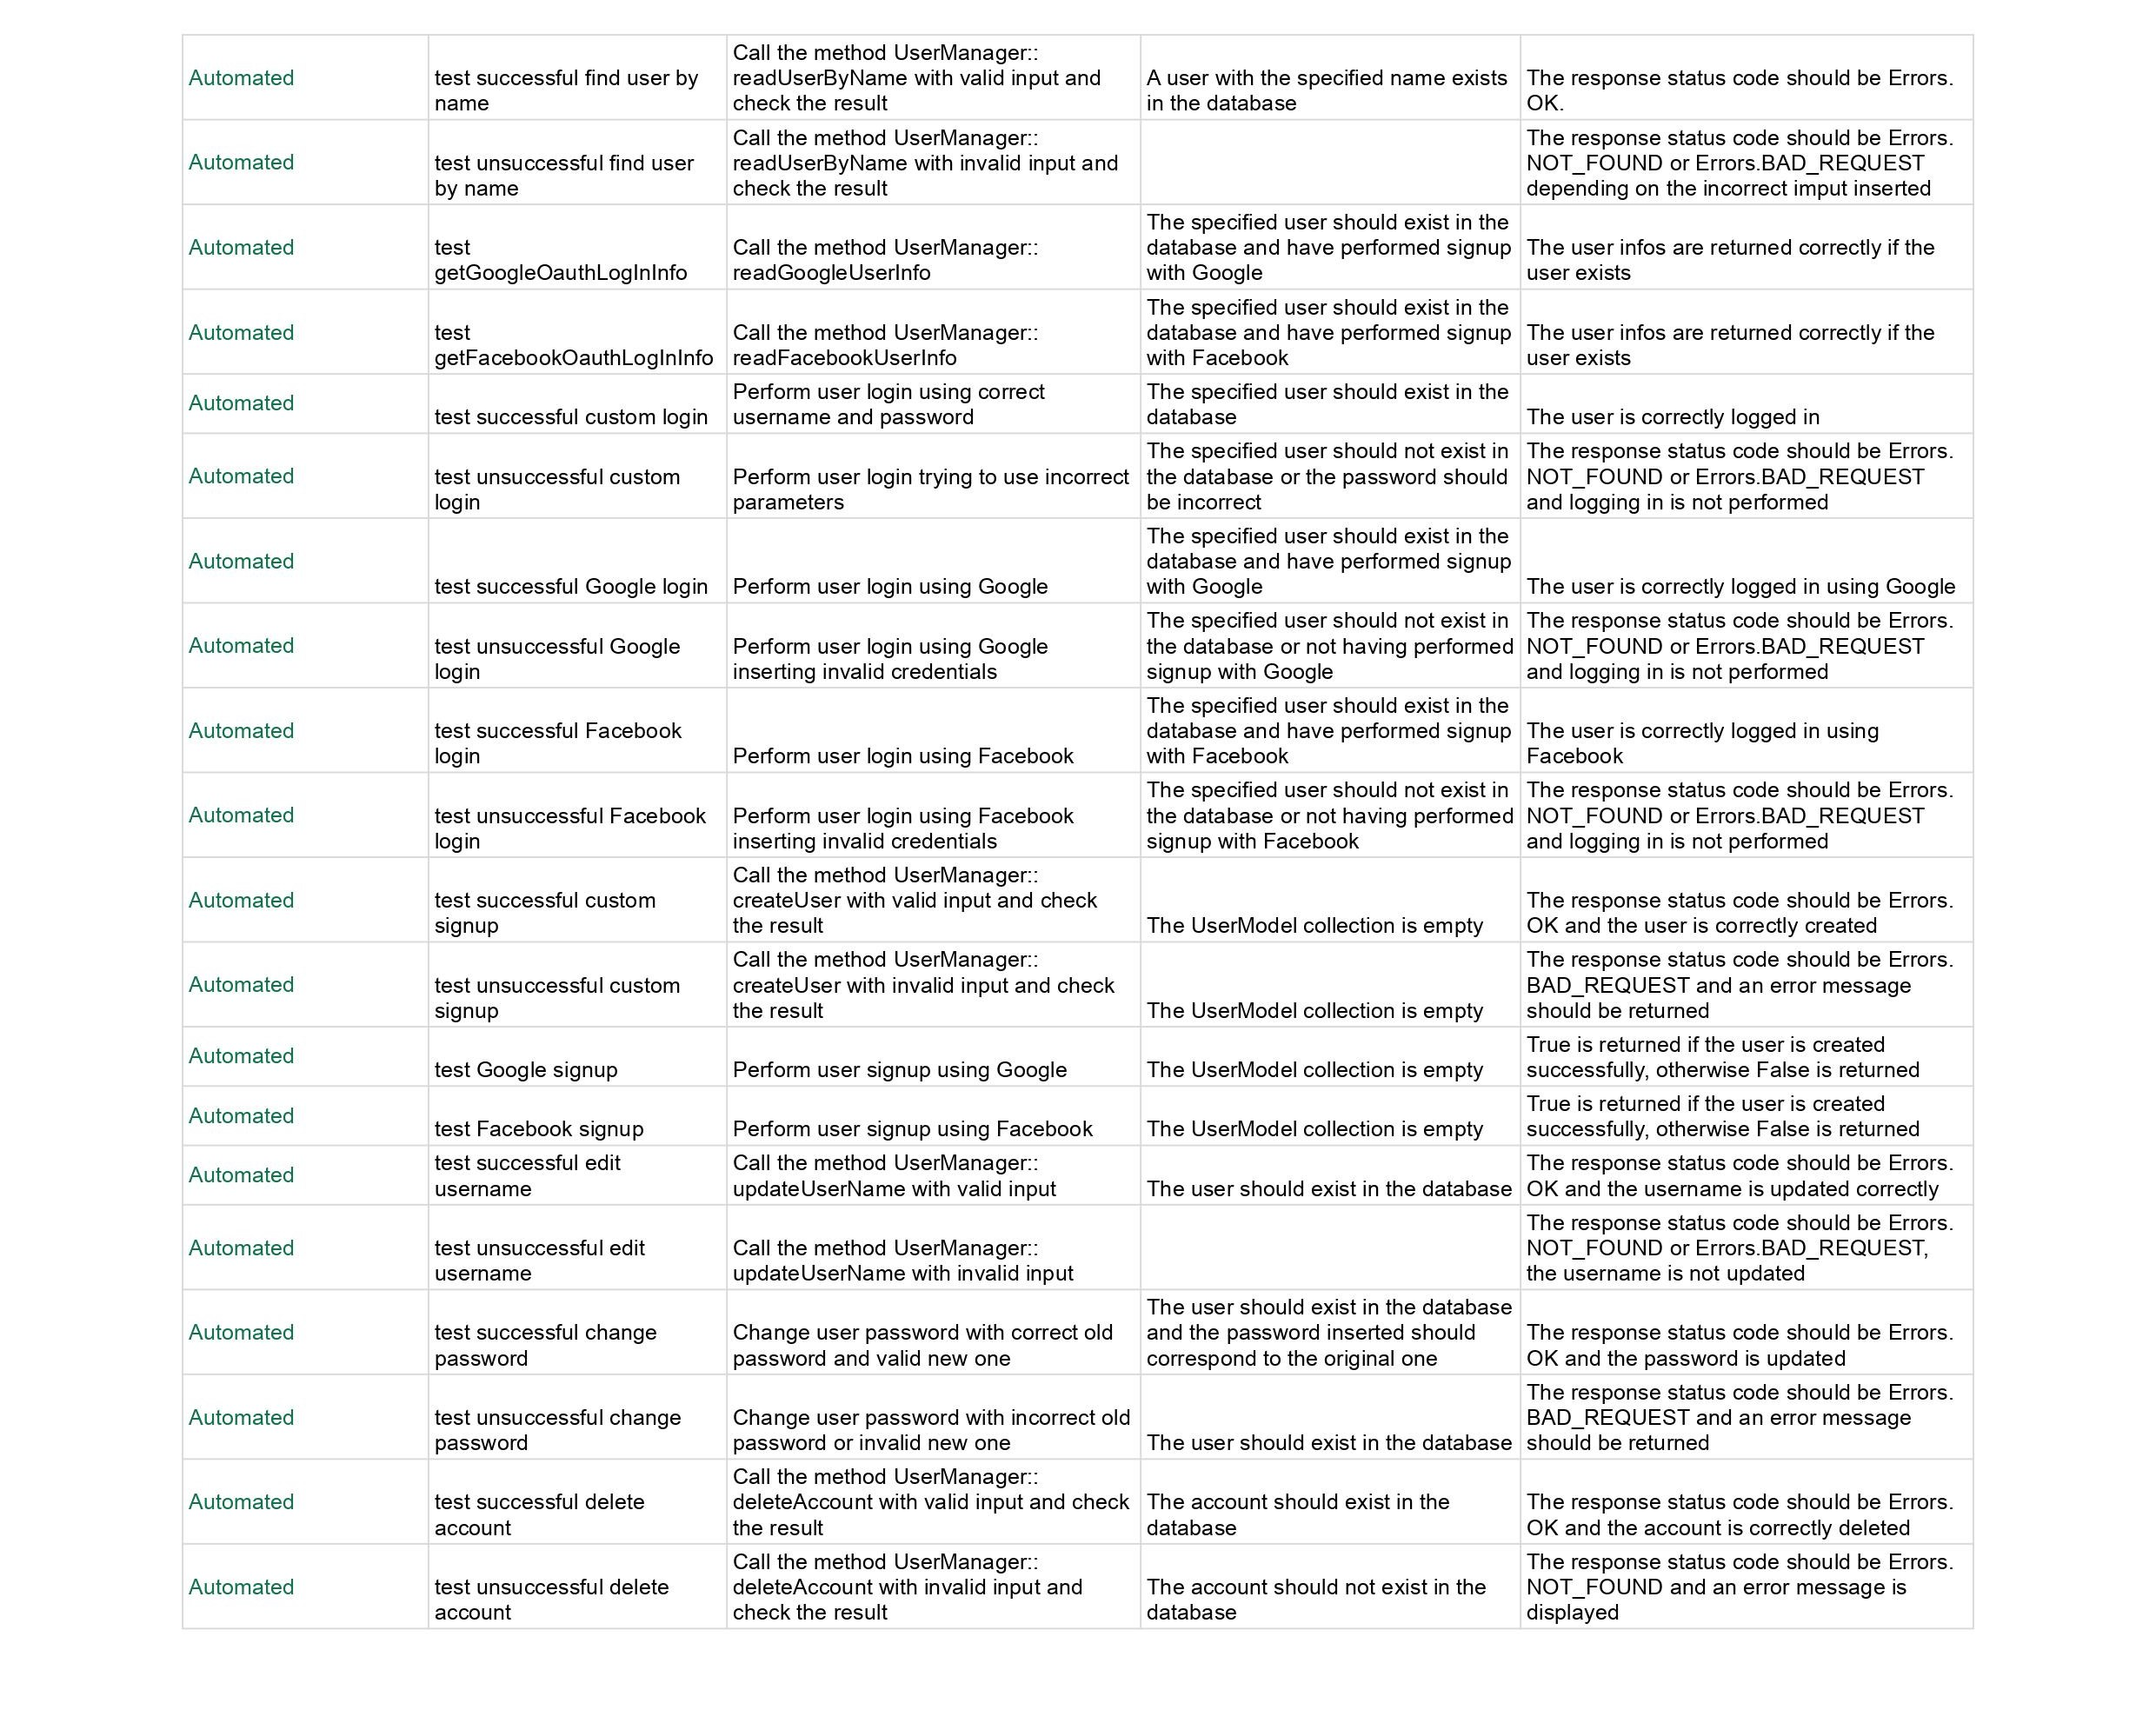
\includegraphics[width=0.95\textwidth]{images/Test_AccountManager.jpg}

\subsection*{Test DatabaseManager::UserManager}
This section is dedicated to the tests for the UserManager class, which is responsible for managing users in the database.
\newline
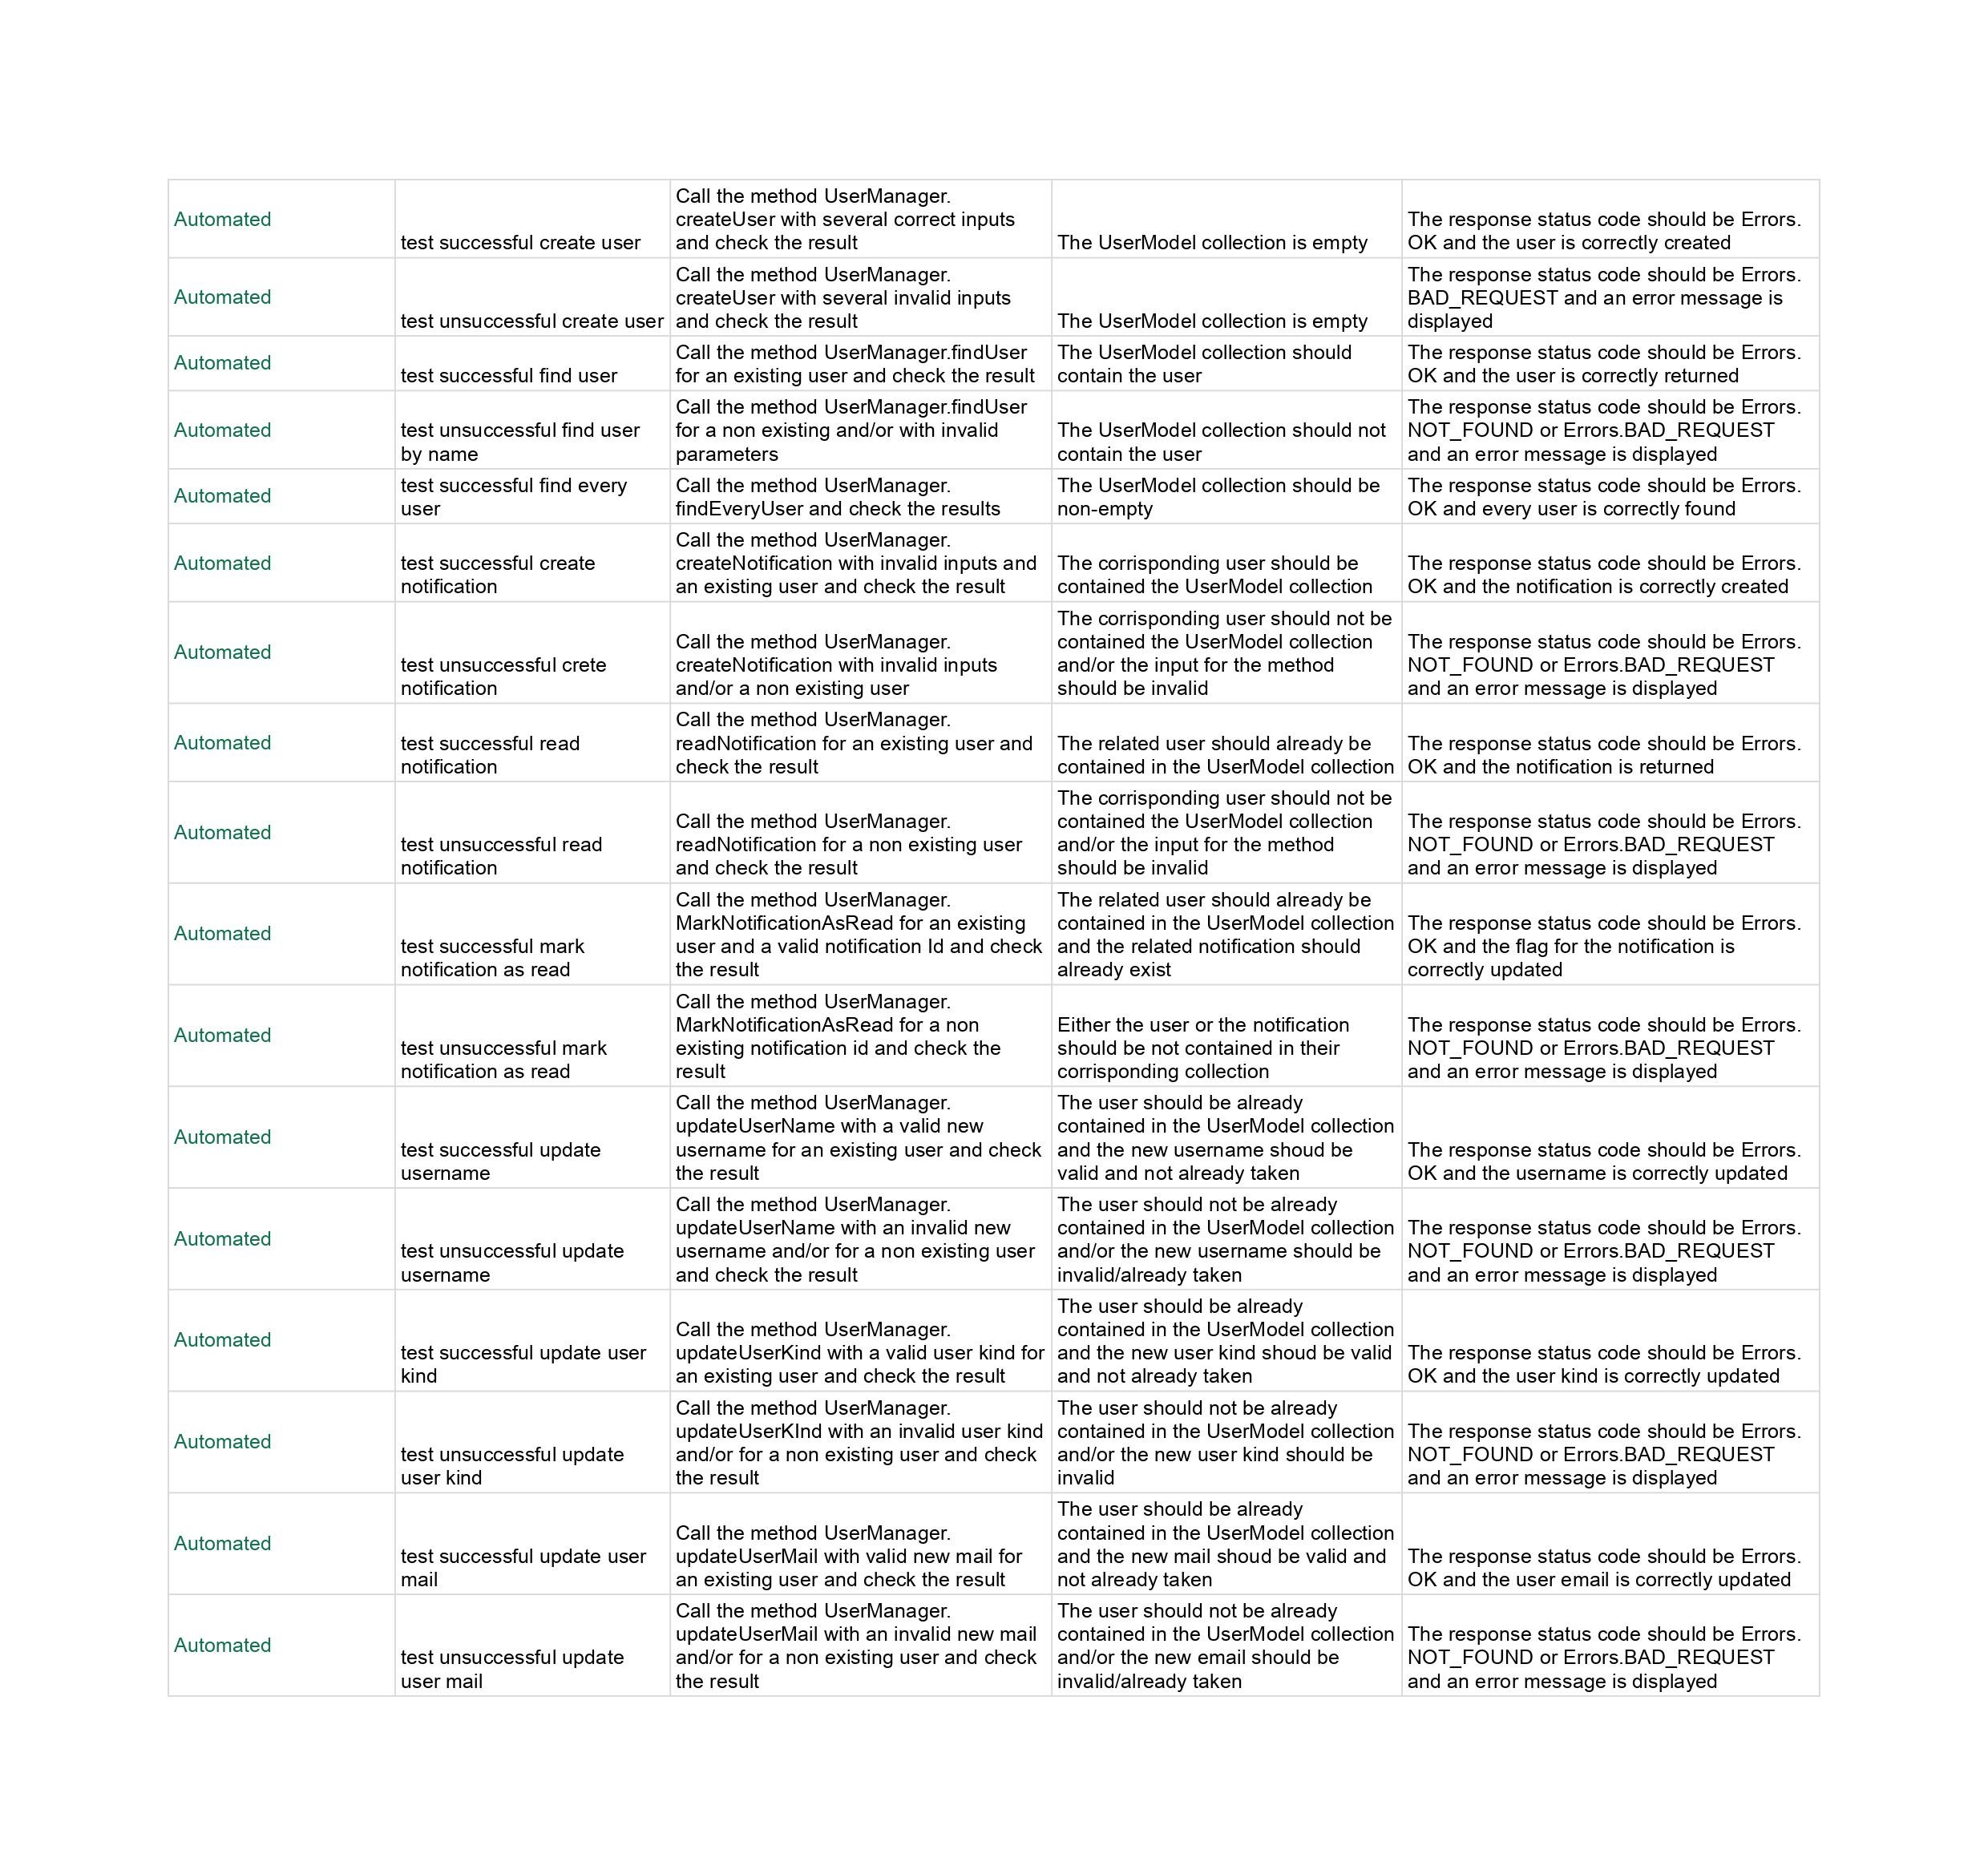
\includegraphics[width=0.95\textwidth]{images/Test_DatabaseManagerUserManager.jpg}

\subsection*{Test TaskManager}
This section includes automated tests for the TaskManager class, which is responsible for managing tasks in the database.
\newline
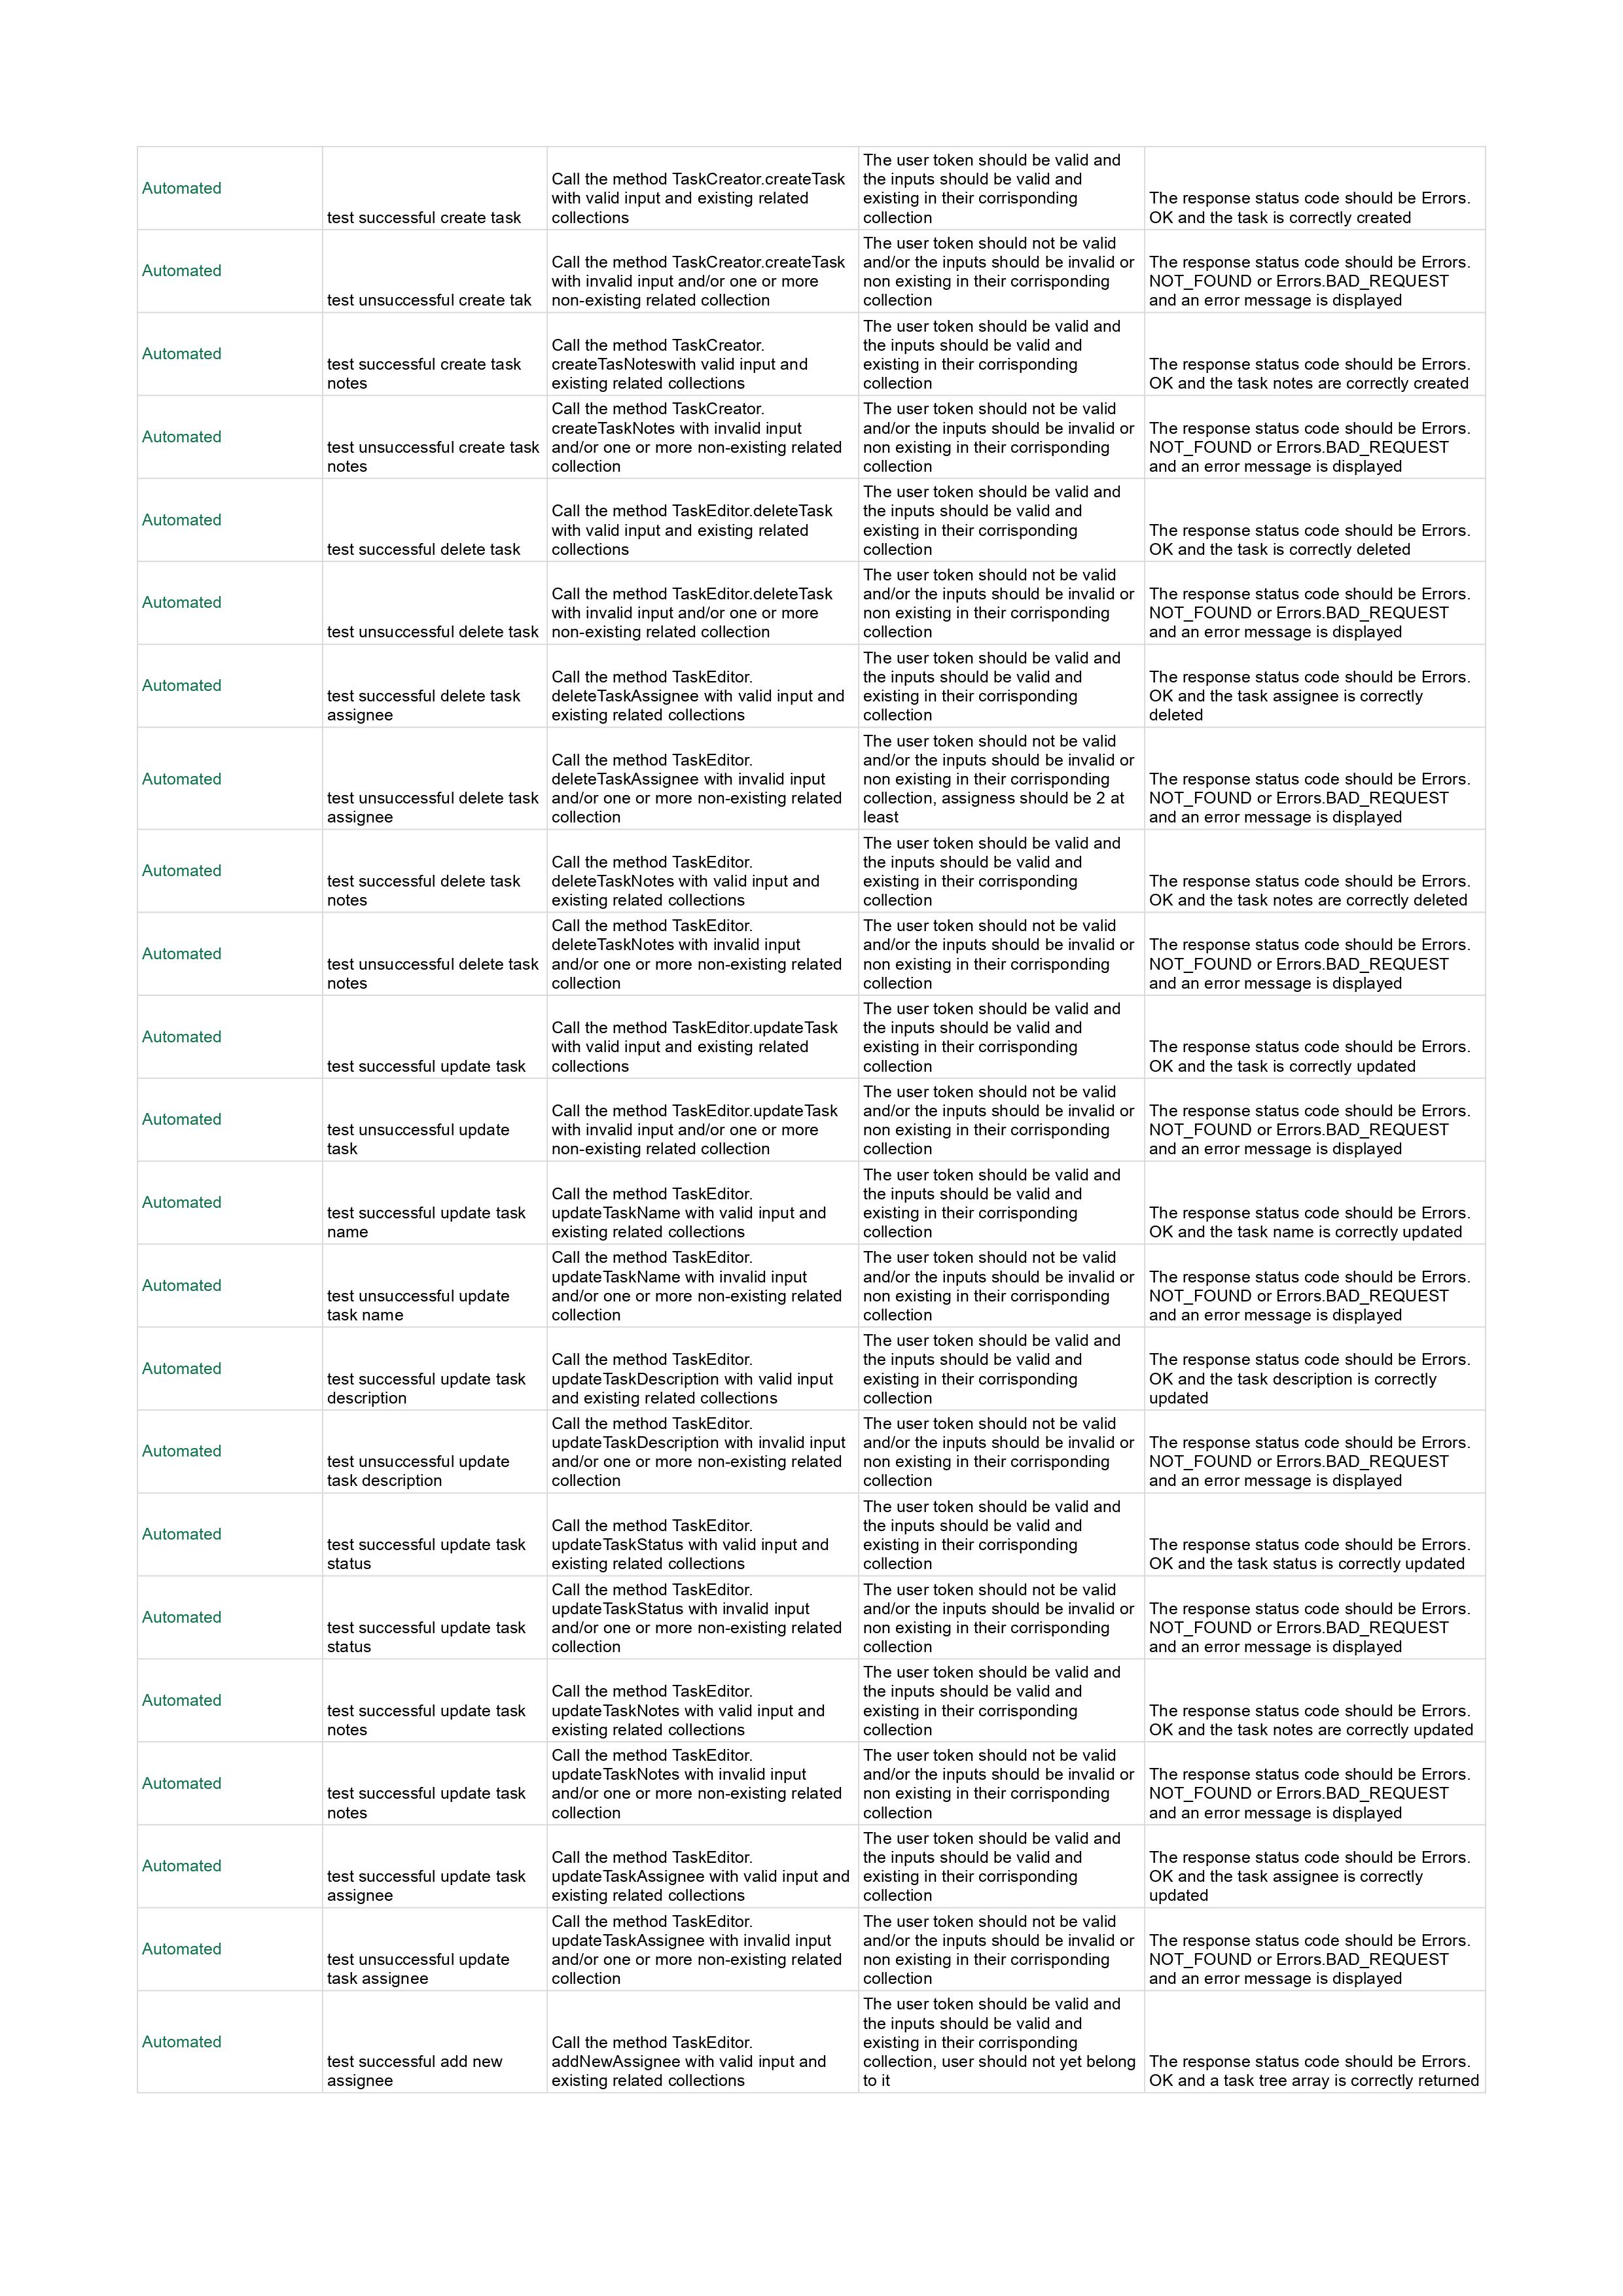
\includegraphics[width=0.95\textwidth]{images/Test_TaskManager-immagini-0.jpg}
\newline
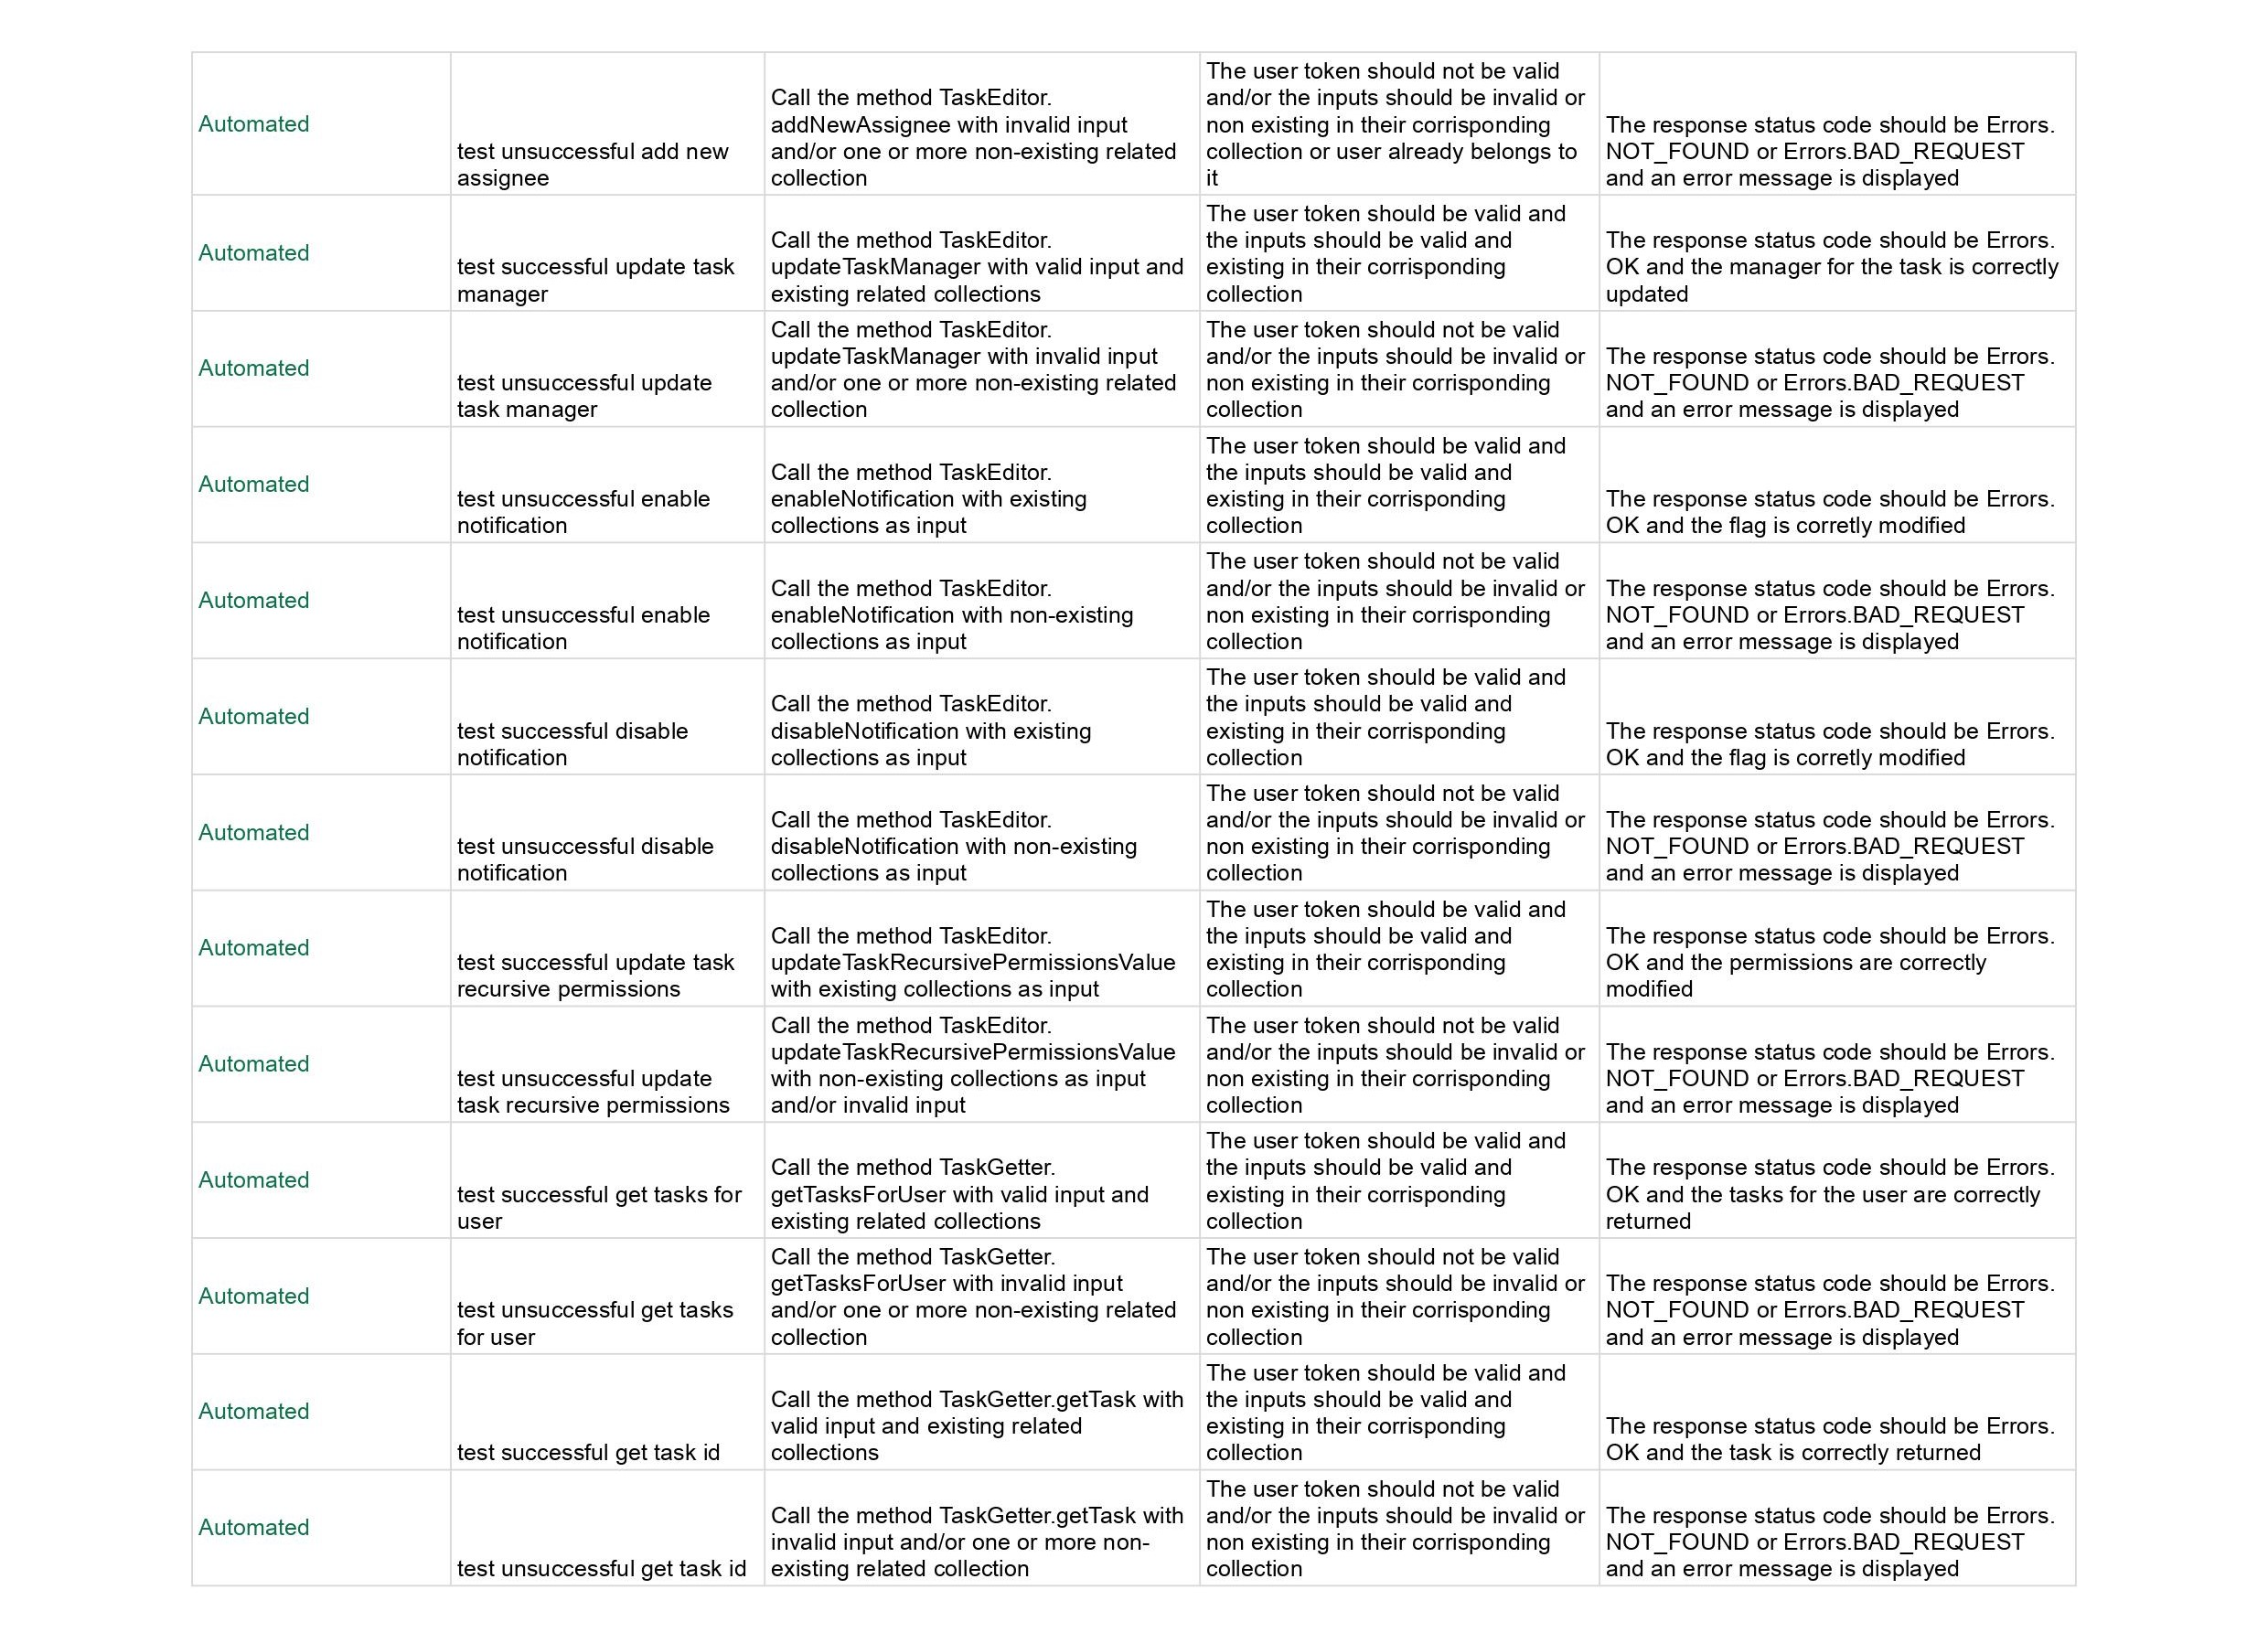
\includegraphics[width=0.95\textwidth]{images/Test_TaskManager-immagini-1.jpg}

\subsection*{Test Home Page}
This section includes manual tests for the home page.
\newline
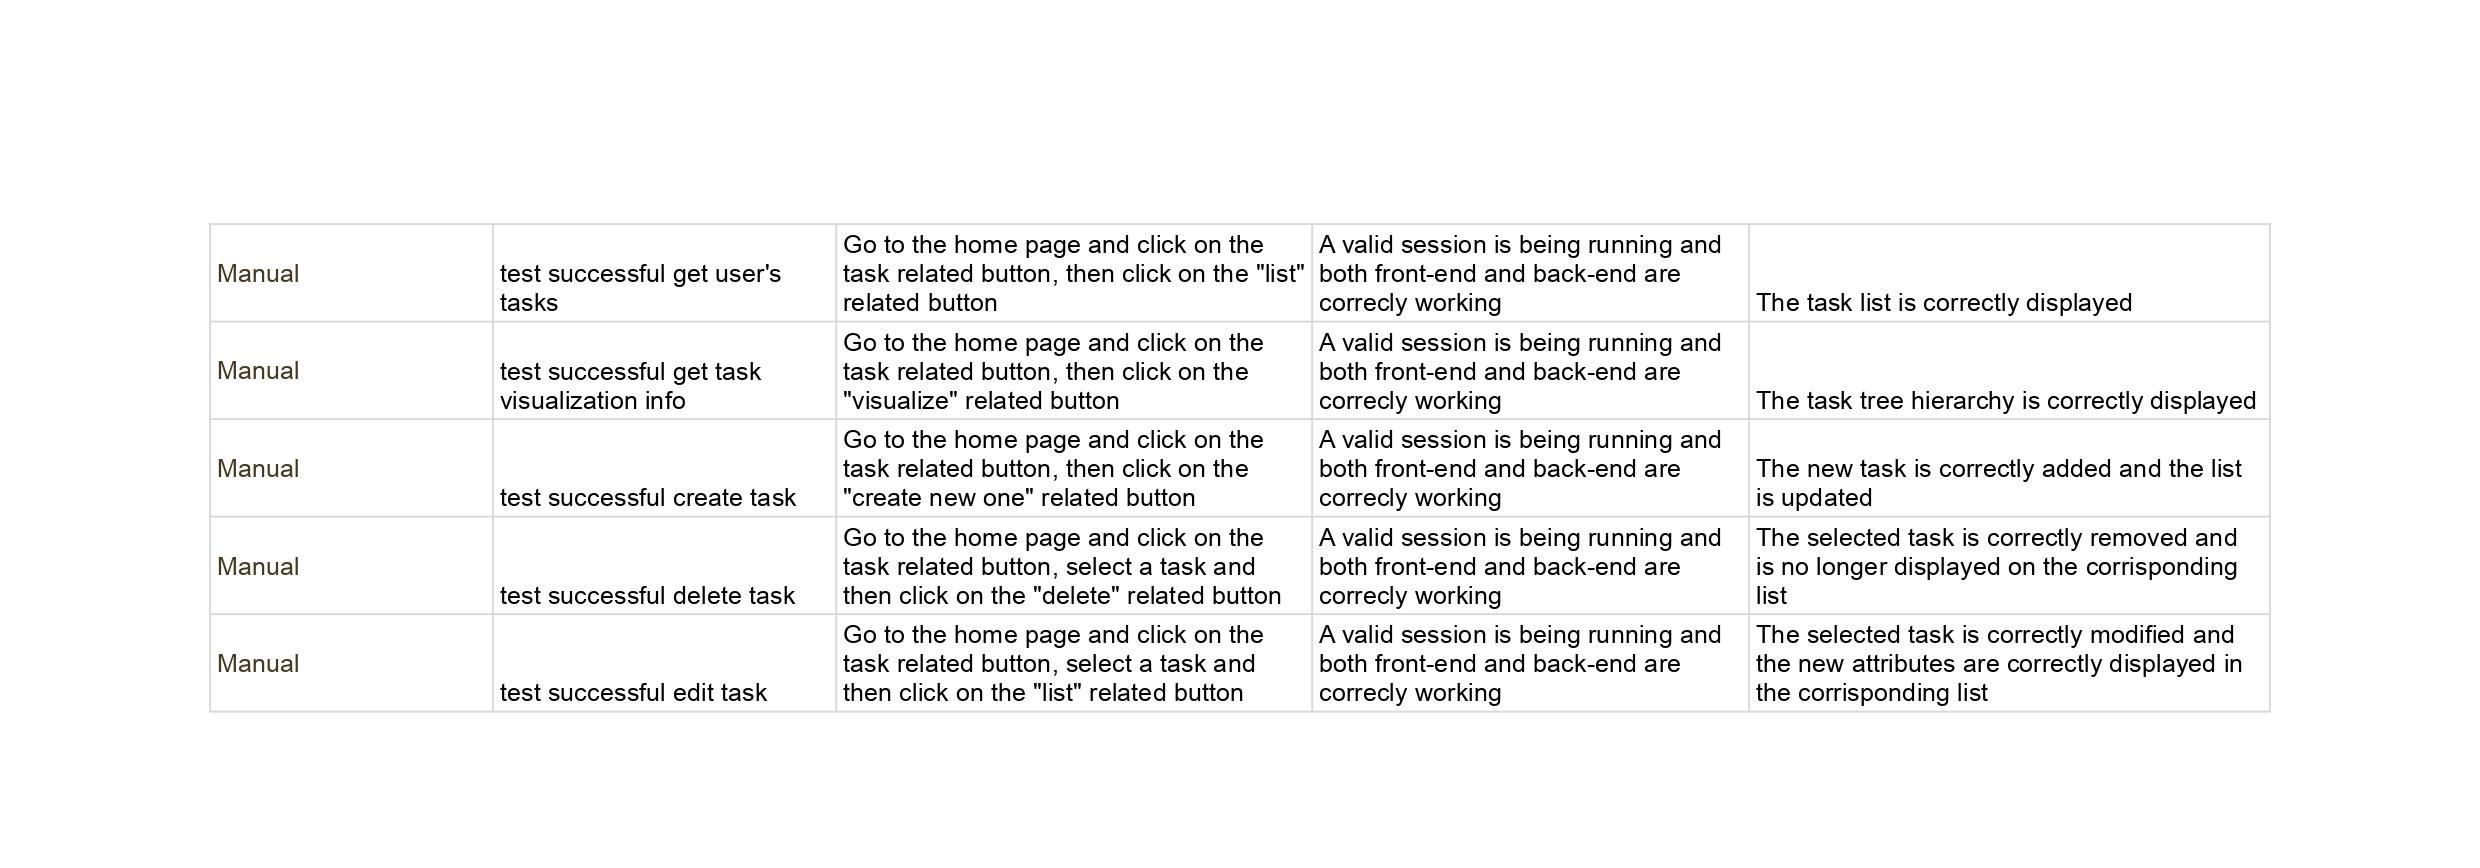
\includegraphics[width=0.95\textwidth]{images/Test_HomePage.jpg}

\subsection*{Test Notification View}
This section includes manual tests for the notification view.
\newline
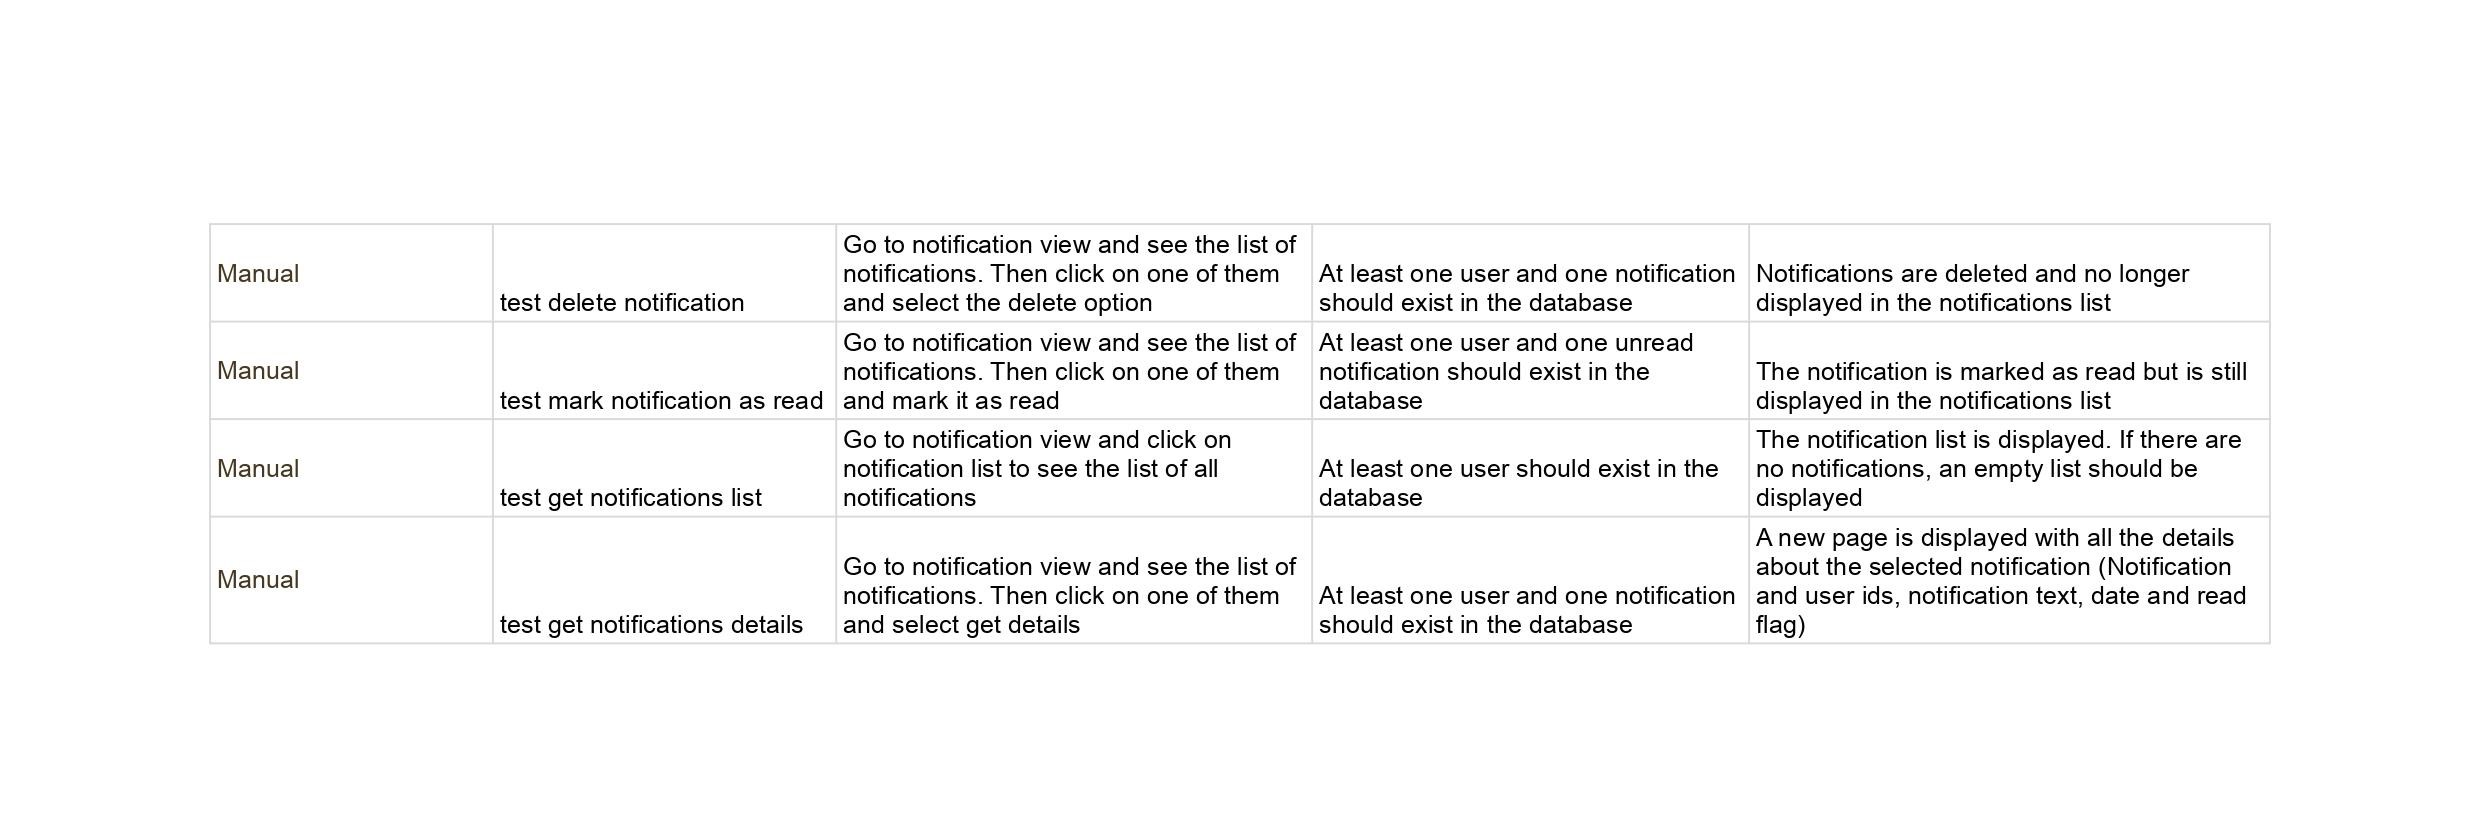
\includegraphics[width=0.95\textwidth]{images/Test_NotificationView.jpg}

\subsection*{Test Sign In and Sign Up Pages}
This section includes manual tests for the sign in and sign up pages.
\newline
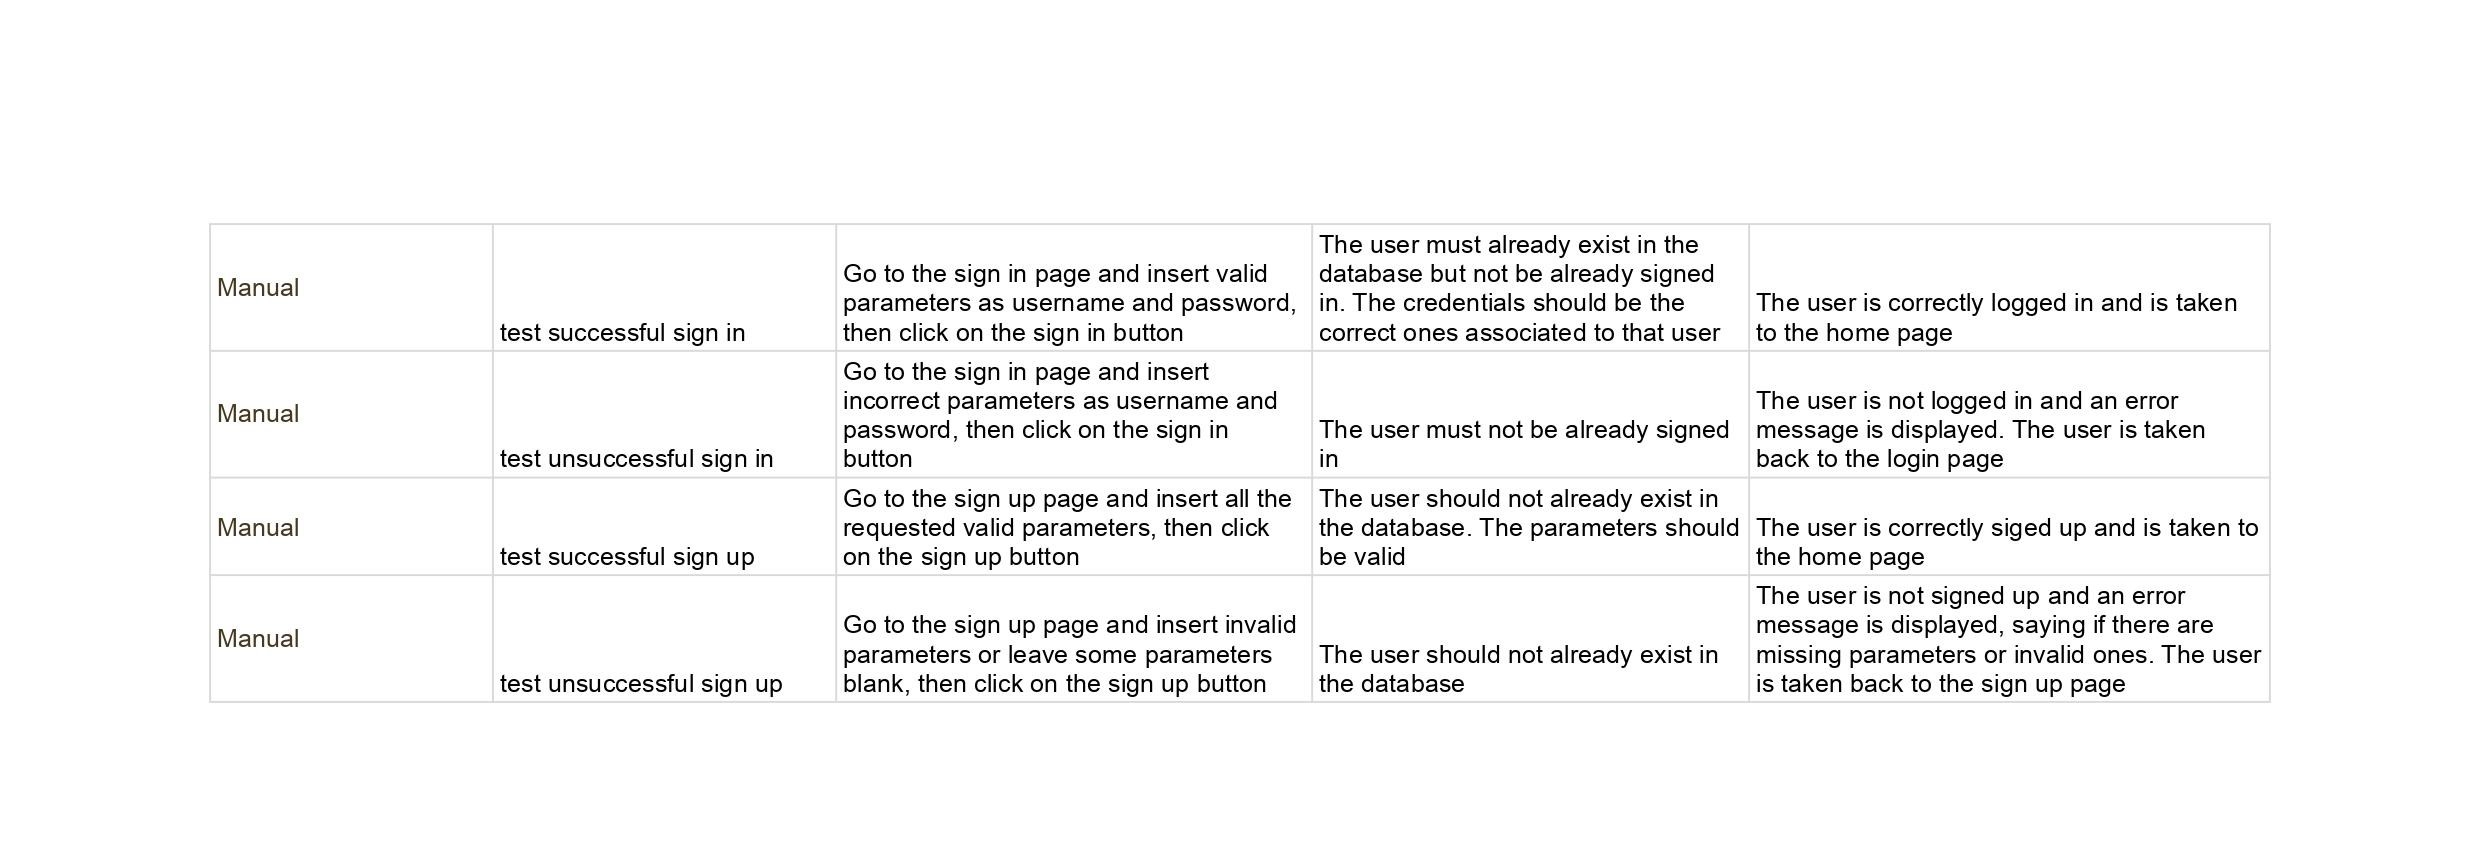
\includegraphics[width=0.95\textwidth]{images/Test_SignInSignUpPage.jpg}

\subsection*{Test Edit Profile Page}
This section includes manual tests for the edit profile page.
\newline
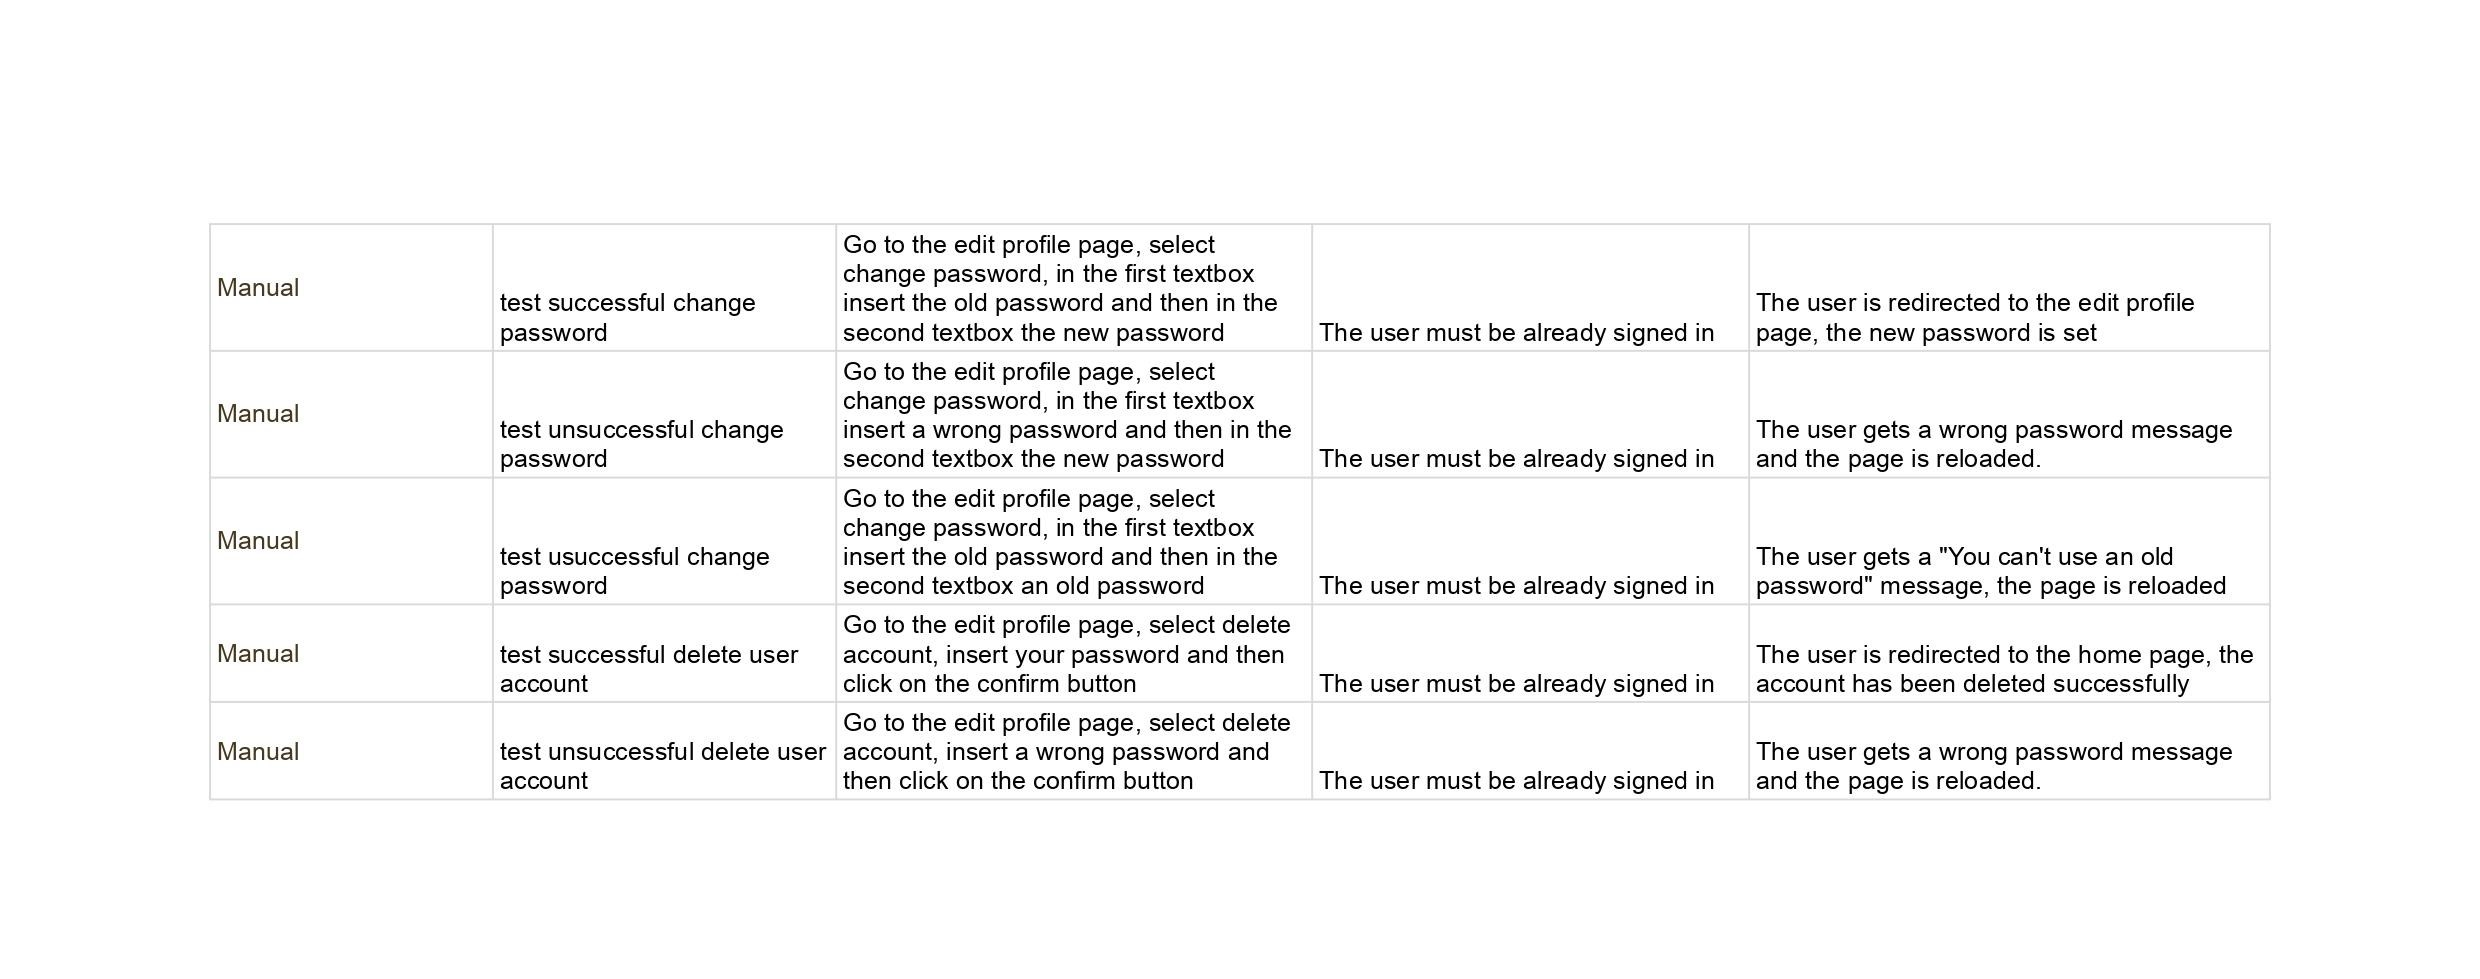
\includegraphics[width=0.95\textwidth]{images/Test_EditProfile.jpg}

\subsection*{Test Organization View Page}
This section includes manual tests for the organization view page.
\newline
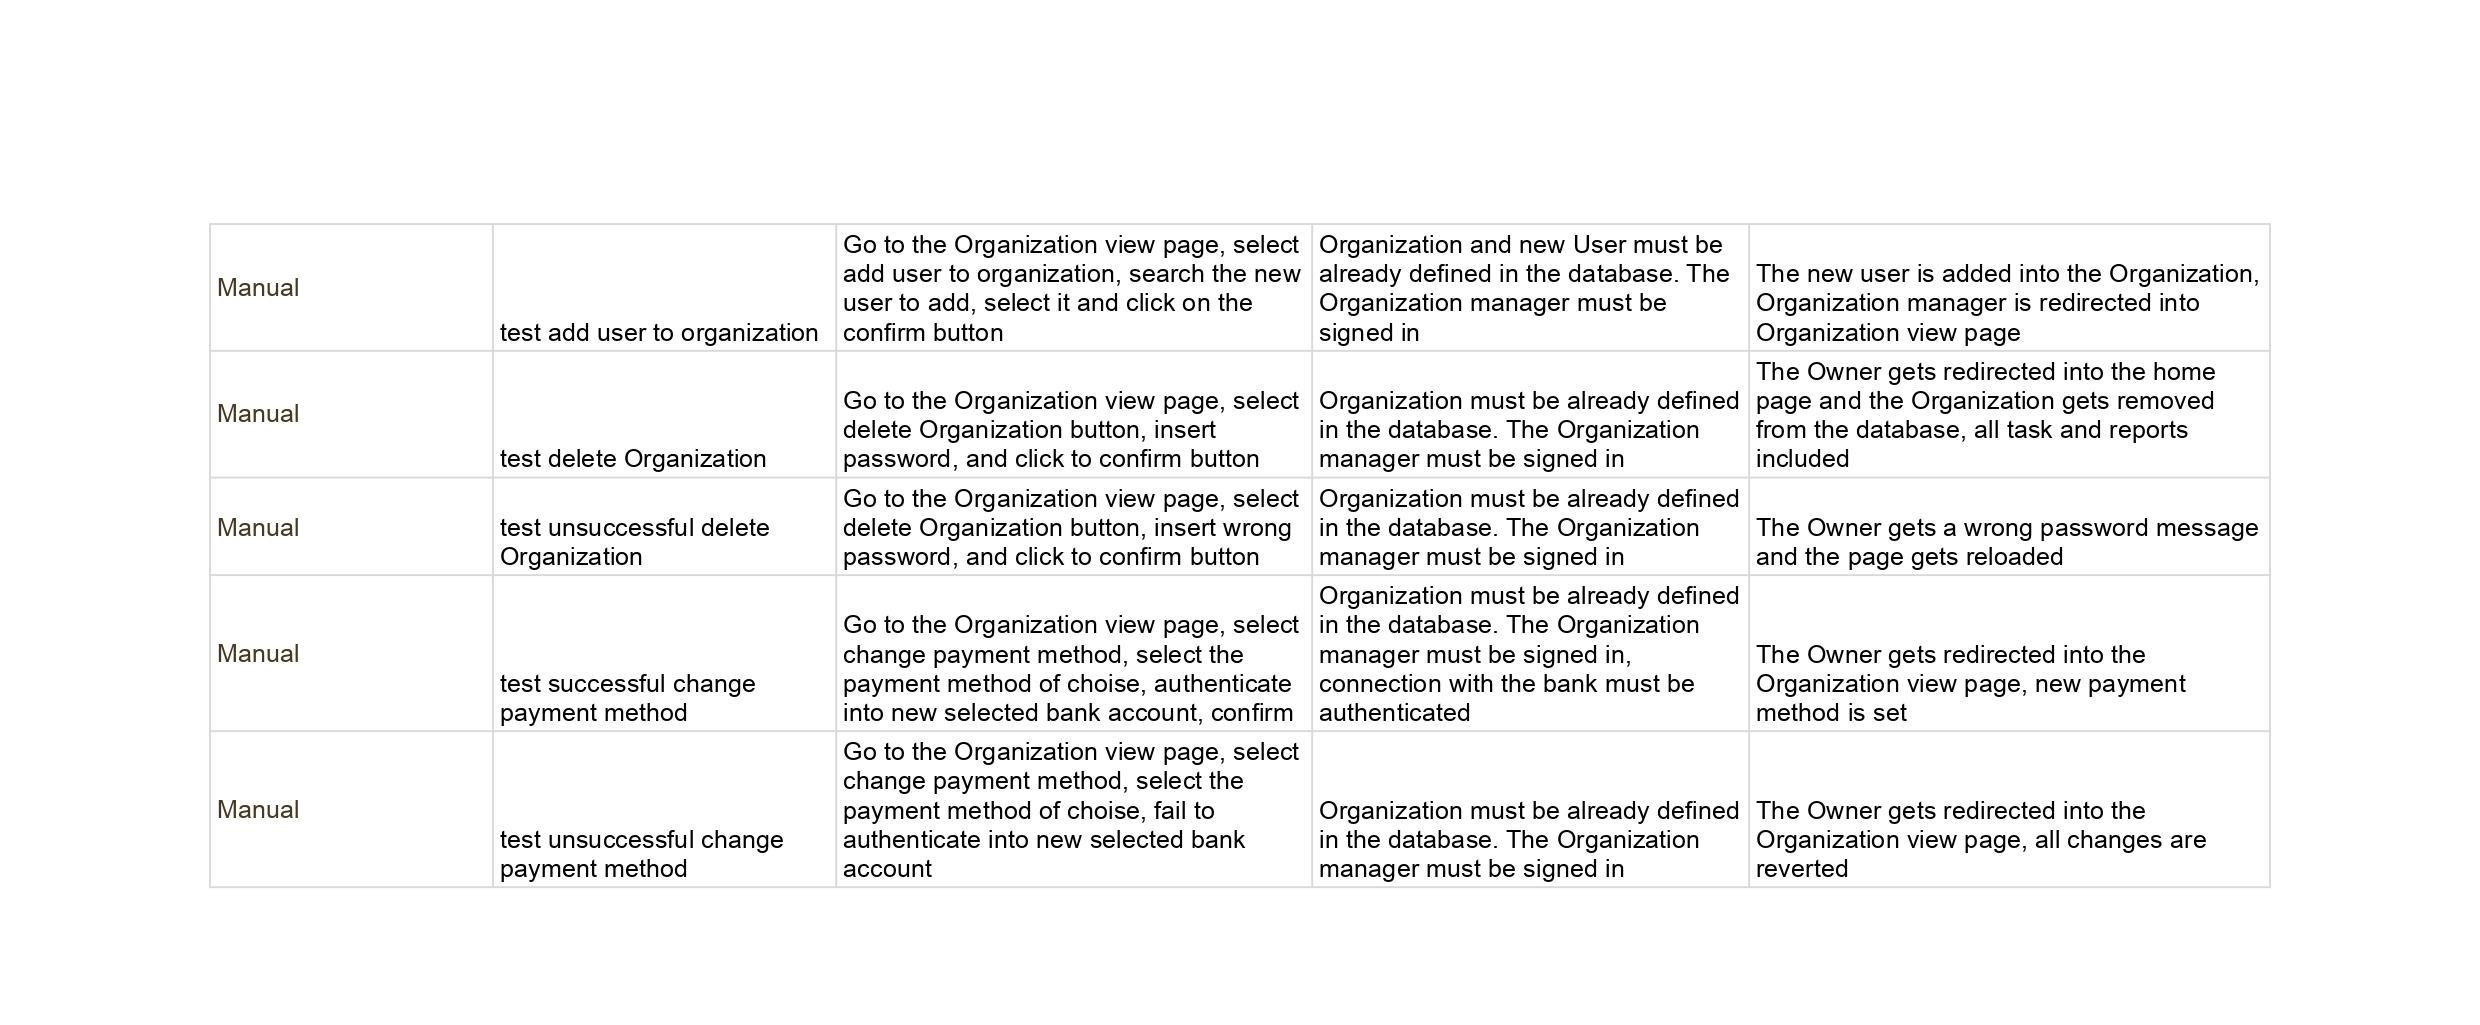
\includegraphics[width=0.95\textwidth]{images/Test_OrganizationView.jpg}

\section{Git Strategy}

We have chosen GitHub Flow as our Git strategy.
We chose it because is one of the simplest strategies and it is suitable for small teams.


\section{Sprint 1}

\subsection{Sprint 1 Backlog}
\includegraphics[width=0.95\textwidth]{images/sprint_backlog.jpg}

\subsection{Sprint 1 Review and Retrospective}

\subsection{Burndown Chart}
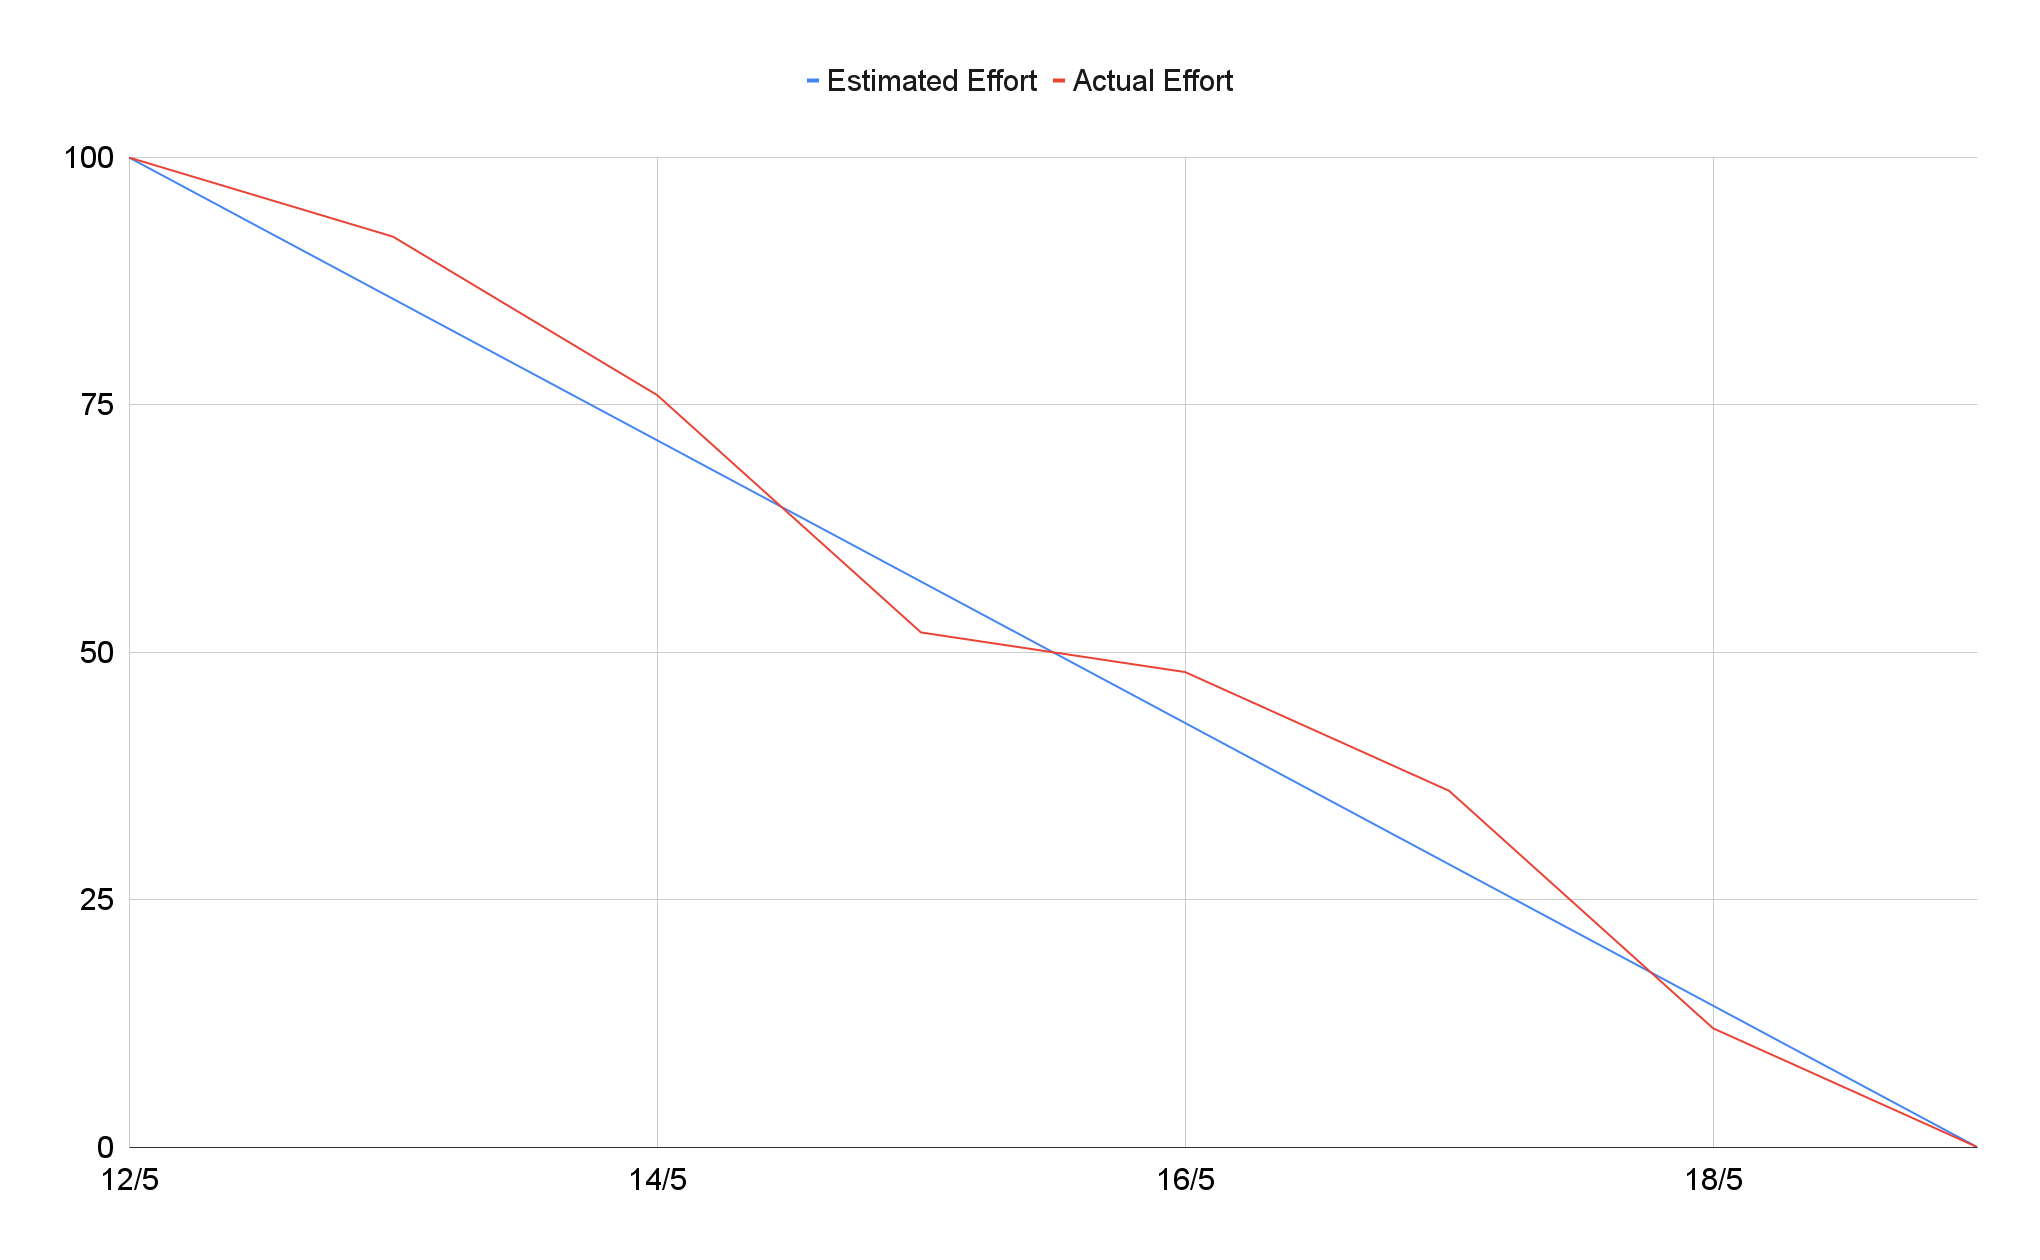
\includegraphics[width=0.95\textwidth]{images/burndown_chart.png}

\end{document}
